%% `prestonh' beamer theme 2017: Main file for compiling
%% Create presentation in `presentation.tex'.
%$ Compile this file. 
%%
%% Color style file for the `prestonh' beamer theme
%% Copyright 2017 Preston Hinkle
%% This file may be distributed and/or modified
%% 	1. under the LaTeX Project Public License and/or
%% 	2. under the GNU Public License.

\documentclass[12 pt]{beamer}
\usetheme[
	bullet=circle,		% Other option: square
	bigpagenumber,		% circled page number on lower right
	topline=true,			% colored bar at the top of the frame 
	shadow=false,			% Shading for beamer blocks
	watermark=watermark.png,
	]{prestonh}



%%%%%%%%%%
% FONTS %
%%%%%%%%%%



%%%%%%%%%%%%%%%%%%%%%%%%
% Usual LaTeX Packages %
%%%%%%%%%%%%%%%%%%%%%%%%

\usepackage{amsmath}
\usepackage{amsfonts}
\usepackage{amssymb}
\usepackage{graphicx}
\usepackage{mathrsfs}							% For Weinberg-esque letters
\usepackage{cancel}							% For "SUSY-breaking" symbol
\usepackage{slashed}							% for slashed characters in math mode
\usepackage{bbm}             						% for \mathbbm{1} (unit matrix)
\usepackage{amsthm}							% For theorem environment
\usepackage{multirow}							% For multi row cells in table
\usepackage{arydshln} 							% For dashed lines in arrays and tables
\usepackage[absolute, overlay]{textpos}		% For absolute positioning of text and pictures
\usepackage{siunitx}
\usepackage{animate}                                                    % For gifs, need adobe acrobat
\usepackage{multimedia}                                                 % For mp4, works on linux with Ocular pdf viewer

\usetikzlibrary{decorations.pathreplacing,calc}



\graphicspath{{images/}}	% Image directory


\usetikzlibrary{backgrounds}
\usetikzlibrary{mindmap,trees}	% For mind map
% http://www.texample.net/tikz/examples/computer-science-mindmap/



\newcommand{\comment}[1]{\textcolor{comment}{\footnotesize{#1}\normalsize}} % comment mild
\newcommand{\Comment}[1]{\textcolor{Comment}{\footnotesize{#1}\normalsize}} % comment bold
\newcommand{\COMMENT}[1]{\textcolor{COMMENT}{\footnotesize{#1}\normalsize}} % comment crazy bold
\newcommand{\Alert}[1]{\textcolor{Alert}{#1}} % louder alert
\newcommand{\ALERT}[1]{\textcolor{ALERT}{#1}} % loudest alert



\author[Preston Hinkle\quad {thinkle@uci.edu}]{Preston Hinkle}
\title[Resistive-pulse sensing for microscale applications
]{Resistive-pulse sensing for microscale applications
}
\institute{University of California, Irvine}
\date{\today}



\begin{document}

% Presets
\setbeamertemplate{itemize/enumerate body begin}{\footnotesize}
\setbeamertemplate{itemize/enumerate subbody begin}{\footnotesize}




%%%%%%%%%%%%%%%%%%%%%%%%%%%%%%%%%%%%%%%%%%%%%%%%%%%%%%%%%%%%%%%%%%%%%%%%%%%%%%%%%%%%%%%%%%%%%%%%%%%%%%%%%%%%%%%%%%%%%%%%%%%%
% Title page
%%%%%%%%%%%%%%%%%%%%%%%%%%%%%%%%%%%%%%%%%%%%%%%%%%%%%%%%%%%%%%%%%%%%%%%%%%%%%%%%%%%%%%%%%%%%%%%%%%%%%%%%%%%%%%%%%%%%%%%%%%%%


% Create background image
{\setbeamertemplate{sidebar right}{\llap{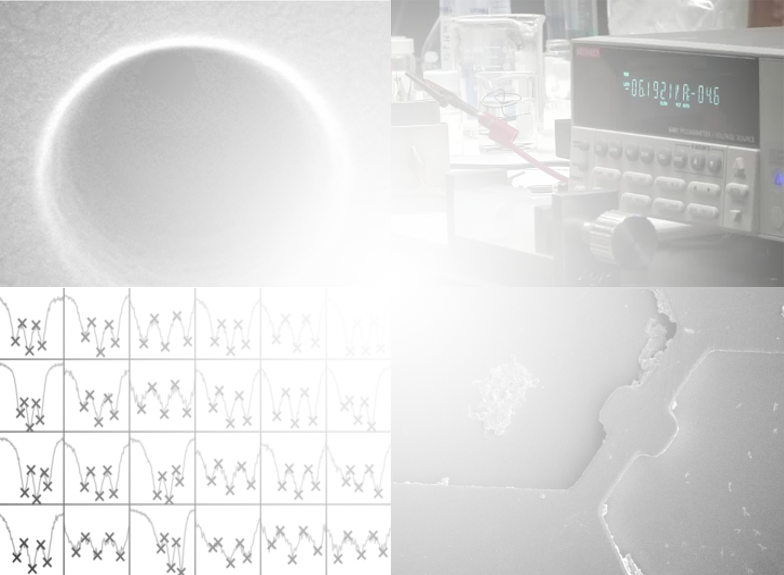
\includegraphics[width=\paperwidth,height=\paperheight]{title_image.png}}}
\begin{frame}[c]
 \begin{center}
  

  
  % Title
  \Huge{
	\textcolor{gray0}{Resistive-pulse sensing at the micro- and nanoscale}
  }
  
  
  % Name --- Institution
  \vspace{.25in}
  {\Large 
	\textcolor{gray1}{Preston Hinkle} \hspace{.5in} 
\includegraphics[height=1em]{uci_wordmark.png}
  }
  
  
  % Talk location
  \vspace{.5in}
  {\small
	\textit{\today}
  }
  
  
  
 \end{center}

\end{frame}
}



%%%%%%%%%%%%%%%%%%%%%%%%%%%%%%%%%%%%%%%%%%%%%%%%%%%%%%%%%%%%%%%%%%%%%%%%%%%%%%%%%%%%%%%%%%%%%%%%%%%%%%%%%%%%%%%%%%%%%%%%%%%%
% Outline
%%%%%%%%%%%%%%%%%%%%%%%%%%%%%%%%%%%%%%%%%%%%%%%%%%%%%%%%%%%%%%%%%%%%%%%%%%%%%%%%%%%%%%%%%%%%%%%%%%%%%%%%%%%%%%%%%%%%%%%%%%%%


\begin{frame}[c]{Outline}
 
	\begin{columns}[t]
		\begin{column}[T]{2.25in}
		
			\setbeamercovered{transparent}
			\begin{itemize}
				\item\only<1>{\textcolor{porestatsblack}{Resistive pulse sensing background}}\only<2,3,4>{\textcolor{ucigray0}{Resistive pulse sensing background}}
				\item\only<2>{\textcolor{porestatsblack}{Resistive pulse sensing of high-aspect ratio particles}}\only<1,3,4>{\textcolor{ucigray0}{Resistive pulse sensing of high-aspect ratio particles}}	
				\item\only<3,4>{\textcolor{porestatsblack}{Microscale resistive pulse sensing}}\only<1,2>{\textcolor{ucigray0}{Microscale resistive pulse sensing}}
				
					\begin{itemize}
						\item\only<3>{\textcolor{porestatsblack}{Simultaneous imaging and resistive pulse studies}}\only<1,2,4>{\textcolor{ucigray0}{Simultaneous imaging and resistive pulse studies}}
						\item\only<4>{\textcolor{porestatsblack}{Cancer cell deformability cytometry}}\only<1,2,3>{\textcolor{ucigray0}{Cancer cell deformability cytometry}}
					\end{itemize}
					
					
				
			\end{itemize}
			\setbeamercovered{invisible}
			
		\end{column}
		
		
		\begin{column}[T]{2.25in}
	
		
			% RP Background 1
			\onslide<1>{
				\begin{picture}(0,0)(0,0)
					\put(0,-180)
					{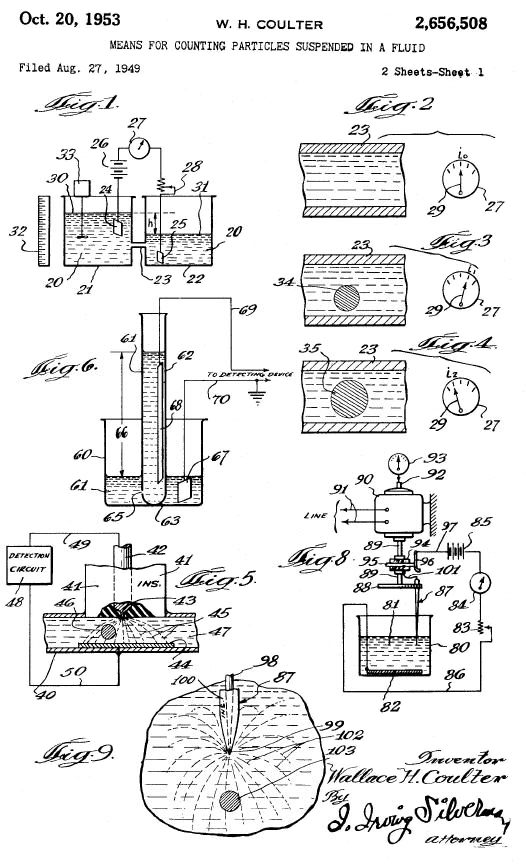
\includegraphics[width=2in]{coulter_patent_drawing}}
				\end{picture}
			}

		
			% Rods 1
			\onslide<2>{
				\begin{picture}(0,0)(0,0)
					\put(10,-30)
					{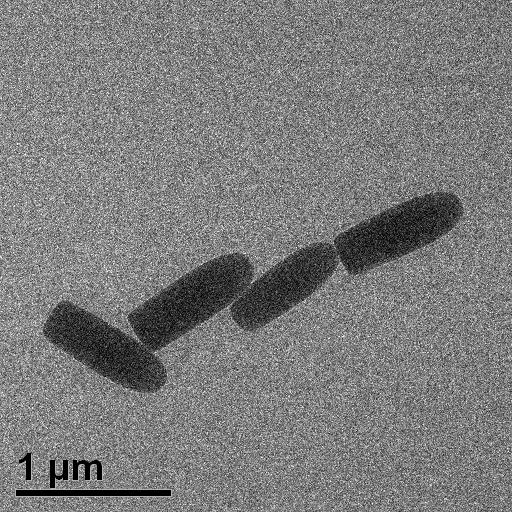
\includegraphics[width=1.25in]{shortrods}}
				\end{picture}
			}
			
			% Rods 2
			\onslide<2>{
				\begin{picture}(0,0)(0,0)
					\put(50,-125)
					{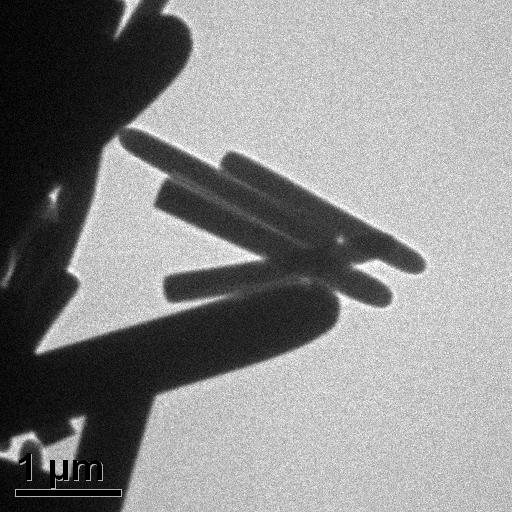
\includegraphics[width=1.25in]{longrods}}
				\end{picture}
			}
			
			
			% RPIM 1
			\onslide<3>{
				\begin{picture}(0,0)(0,0)
					\put(0, -65)
					{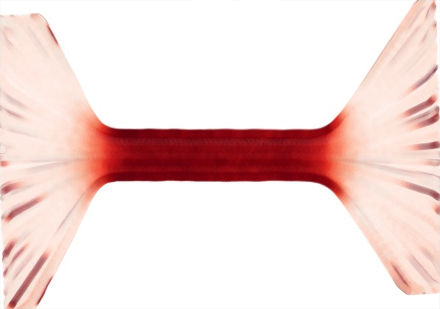
\includegraphics[width=2.25in]{resistancemap}}
				\end{picture}
			}
			
			% Cells
			\onslide<4>{
				\begin{picture}(0,0)(0,0)
					\put(0, -75)
					{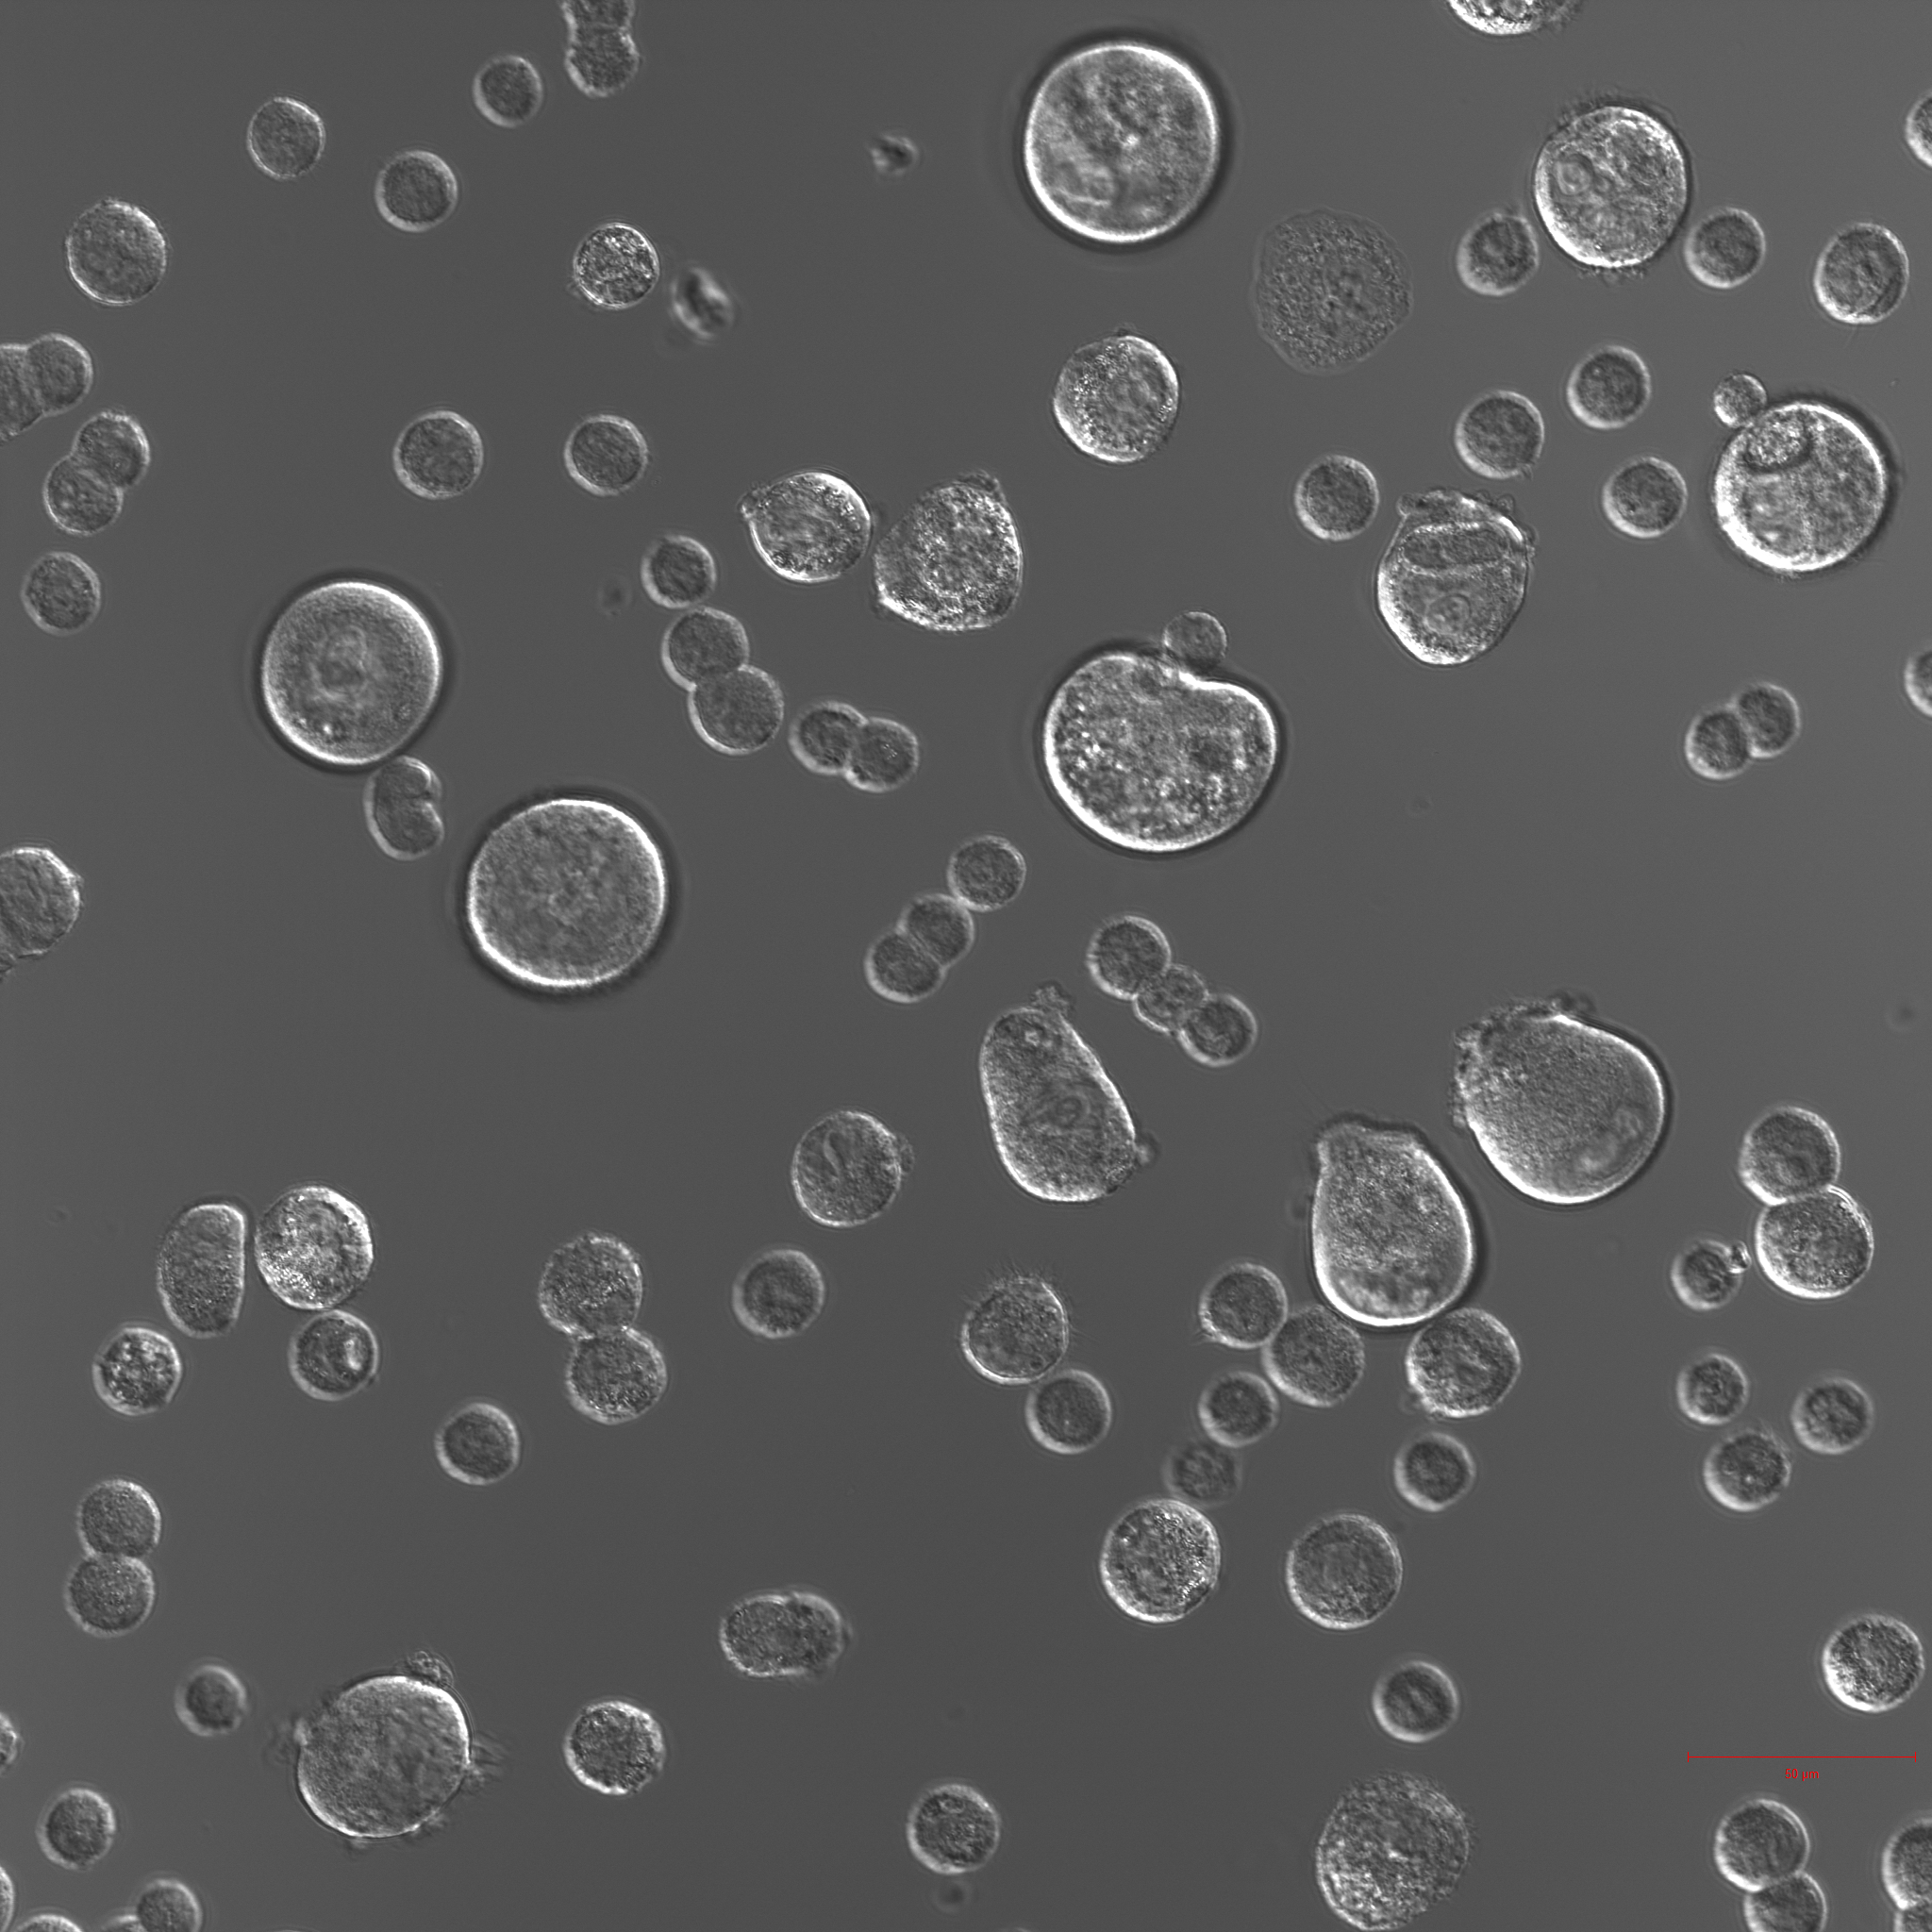
\includegraphics[width=2.25in]{cells}}
				\end{picture}
			}


			
			
		\end{column}
		
	\end{columns}

	
	
	
	
	
\end{frame}


%%%%%%%%%%%%%%%%%%%%%%%%%%%%%%%%%%%%%%%%%%%%%%%%%%%%%%%%%%%%%%%%%%%%%%%%%%%%%%%%%%%%%%%%%%%%%%%%%%%%%%%%%%%%%%%%%%%%%%%%%%%%
% Resistive pulse background title slide
%%%%%%%%%%%%%%%%%%%%%%%%%%%%%%%%%%%%%%%%%%%%%%%%%%%%%%%%%%%%%%%%%%%%%%%%%%%%%%%%%%%%%%%%%%%%%%%%%%%%%%%%%%%%%%%%%%%%%%%%%%%%


\begin{frame}[c]{}
	\begin{center}
		\textbf{Resistive pulse sensing background}
	\end{center}
\end{frame}



%%%%%%%%%%%%%%%%%%%%%%%%%%%%%%%%%%%%%%%%%%%%%%%%%%%%%%%%%%%%%%%%%%%%%%%%%%%%%%%%%%%%%%%%%%%%%%%%%%%%%%%%%%%%%%%%%%%%%%%%%%%%
% Resistive pulse background---description
%%%%%%%%%%%%%%%%%%%%%%%%%%%%%%%%%%%%%%%%%%%%%%%%%%%%%%%%%%%%%%%%%%%%%%%%%%%%%%%%%%%%%%%%%%%%%%%%%%%%%%%%%%%%%%%%%%%%%%%%%%%%


\begin{frame}[c]{Resistive pulse sensing---description}
	
	\begin{columns}[t]
		\begin{column}[T]{2.75in}
	
			\begin{itemize}
				\item Resistive pulse sensing (RP) is a method for single particle detection and characterization
				\item Works at any scale (nano, micro, milli, etc.)
				\item A diverse range of applications: red blood cell counting (several $\SI{}{\mu m}$, virus detection ($10-\SI{100}{\mu m}$, and DNA sequencing ($\sim\SI{1}{nm}$), among others
			\end{itemize}
	
		\end{column}
		
		\begin{column}[T]{1.75in}
			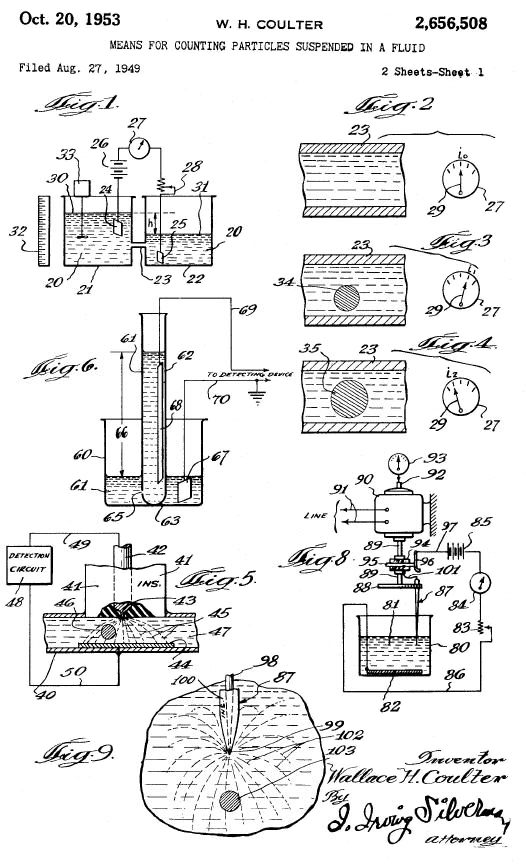
\includegraphics[width=1.75in]{coulter_patent_drawing.png}
		\end{column}
		
	\end{columns}

	
\end{frame}



%%%%%%%%%%%%%%%%%%%%%%%%%%%%%%%%%%%%%%%%%%%%%%%%%%%%%%%%%%%%%%%%%%%%%%%%%%%%%%%%%%%%%%%%%%%%%%%%%%%%%%%%%%%%%%%%%%%%%%%%%%%%
% Resistive pulse background---how does it work?
%%%%%%%%%%%%%%%%%%%%%%%%%%%%%%%%%%%%%%%%%%%%%%%%%%%%%%%%%%%%%%%%%%%%%%%%%%%%%%%%%%%%%%%%%%%%%%%%%%%%%%%%%%%%%%%%%%%%%%%%%%%%


\begin{frame}[c]{Resistive pulse sensing---how does it work?}

	\begin{columns}[t]
		\begin{column}[T]{2.75in}
	      
	

			\begin{tiny}
				\begin{itemize}
				
					\item A nanopore immersed in electrolyte solution acts as an ionic resistor
					\item Current-Voltage relationship follows Ohm's law $V=IR$
					\item When a particle enters the channel its resistance changes, yielding a pulse in the measured ionic current
					\item Pulse properties yield information on size, shape, charge, and concentration of particle
				\end{itemize}
			\end{tiny}
			
		\end{column}
		
		\begin{column}[T]{1.75in}
			{\centering
				\vspace{.5cm}
				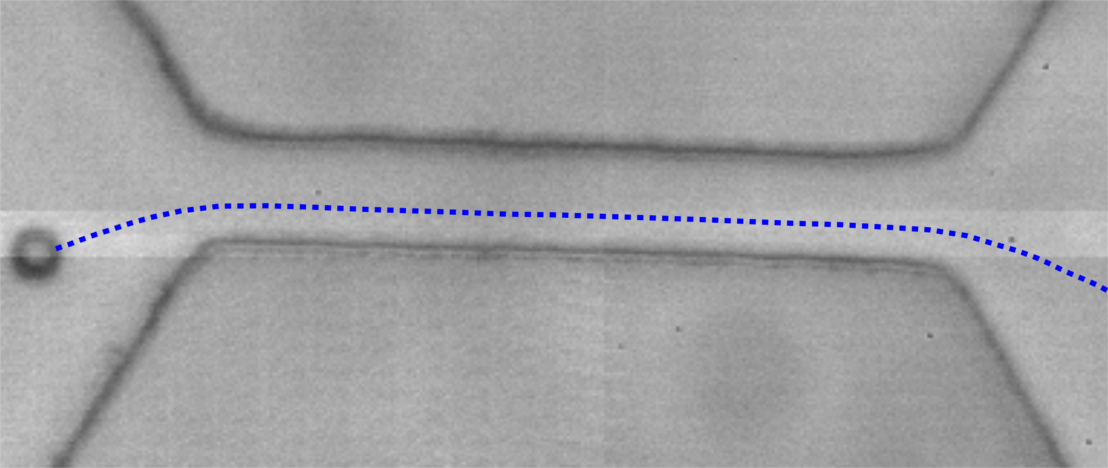
\includegraphics[width=1.5in]{singletrajectory} \\
				\vspace{.75cm}
				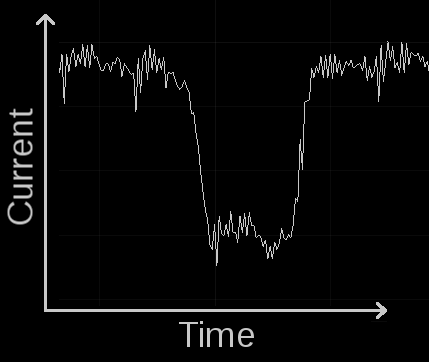
\includegraphics[width=1.5in]{singlerp} \\
				\par
			}
			
		\end{column}

	
	
	\end{columns}
	
\end{frame}




%%%%%%%%%%%%%%%%%%%%%%%%%%%%%%%%%%%%%%%%%%%%%%%%%%%%%%%%%%%%%%%%%%%%%%%%%%%%%%%%%%%%%%%%%%%%%%%%%%%%%%%%%%%%%%%%%%%%%%%%%%%%
% Resistive pulse background---system components
%%%%%%%%%%%%%%%%%%%%%%%%%%%%%%%%%%%%%%%%%%%%%%%%%%%%%%%%%%%%%%%%%%%%%%%%%%%%%%%%%%%%%%%%%%%%%%%%%%%%%%%%%%%%%%%%%%%%%%%%%%%%


\begin{frame}[c]{Resistive pulse sensing---system components}
	%\begin{picture}(0,0)(0,0)
		%\put(90,-125){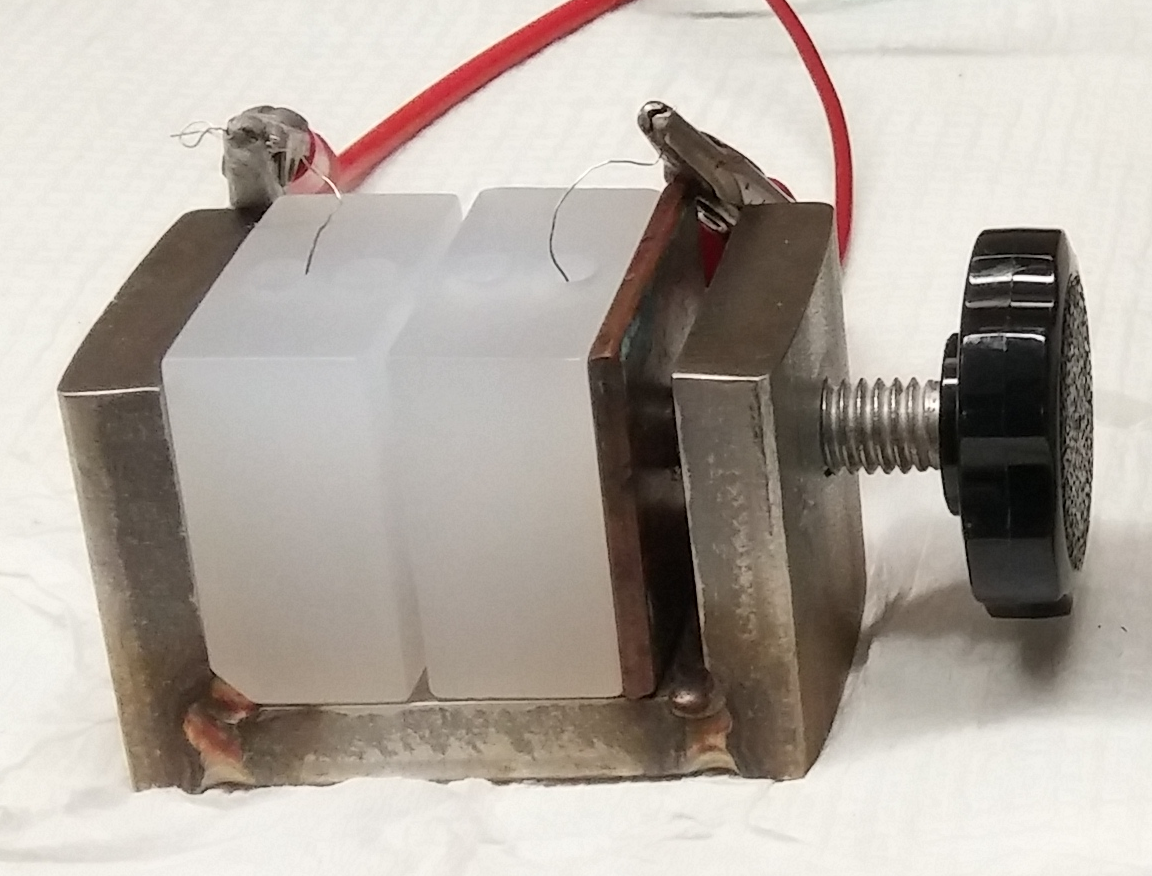
\includegraphics[width=7cm]{photo/conductivitycell.png}}
		%\put(100,0){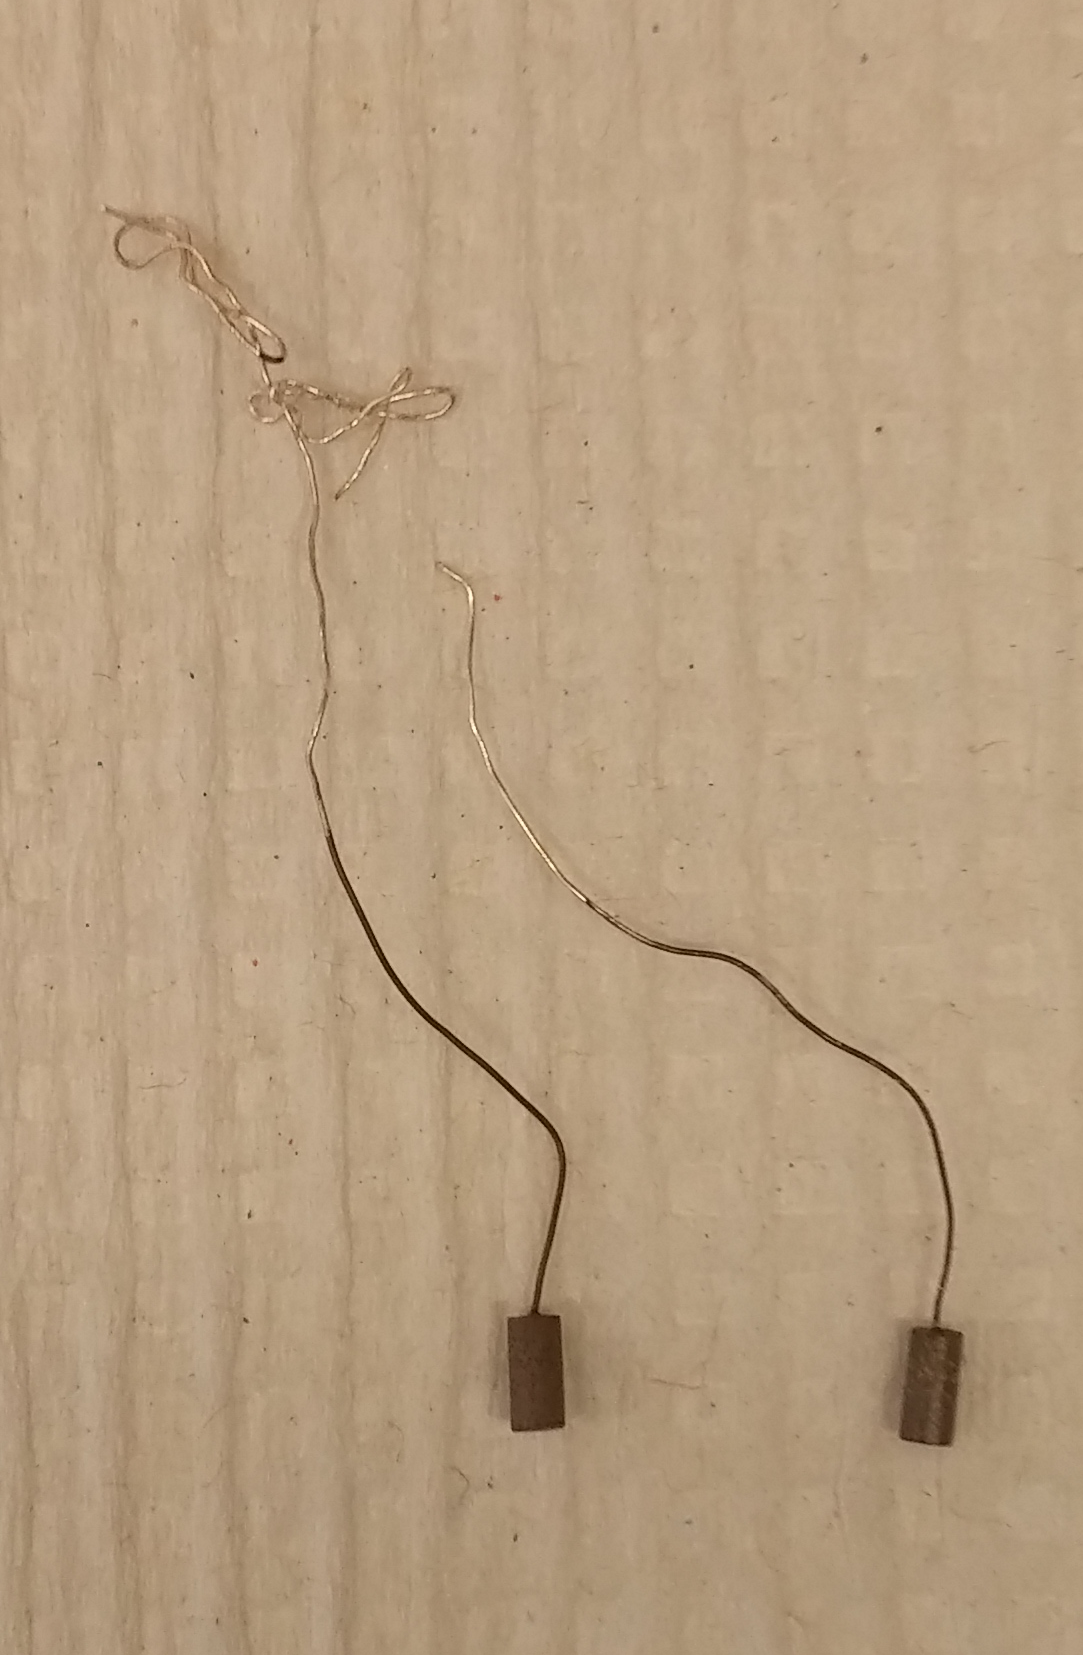
\includegraphics[width=2cm]{photo/electrodes.png}}
		%\put(10,-20){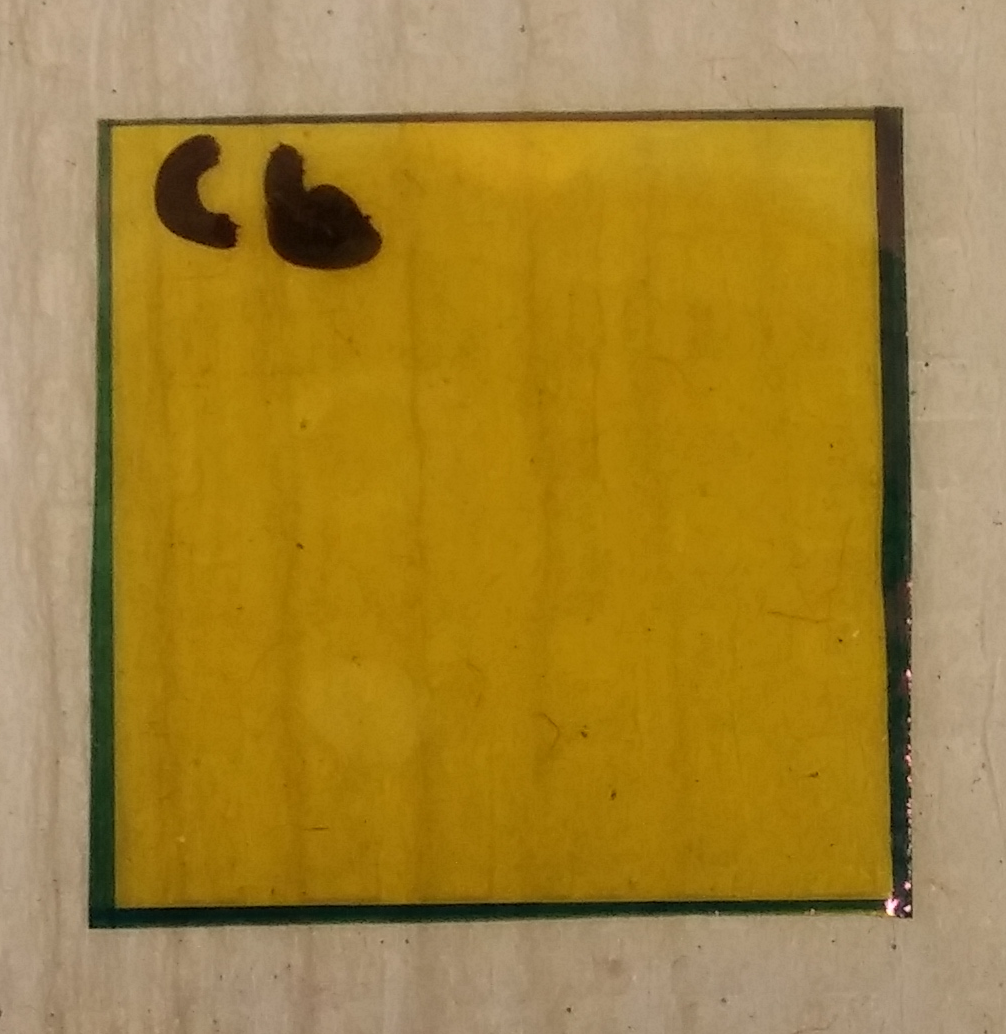
\includegraphics[width=2cm]{photo/membrane.png}}
		%\put(30,-80){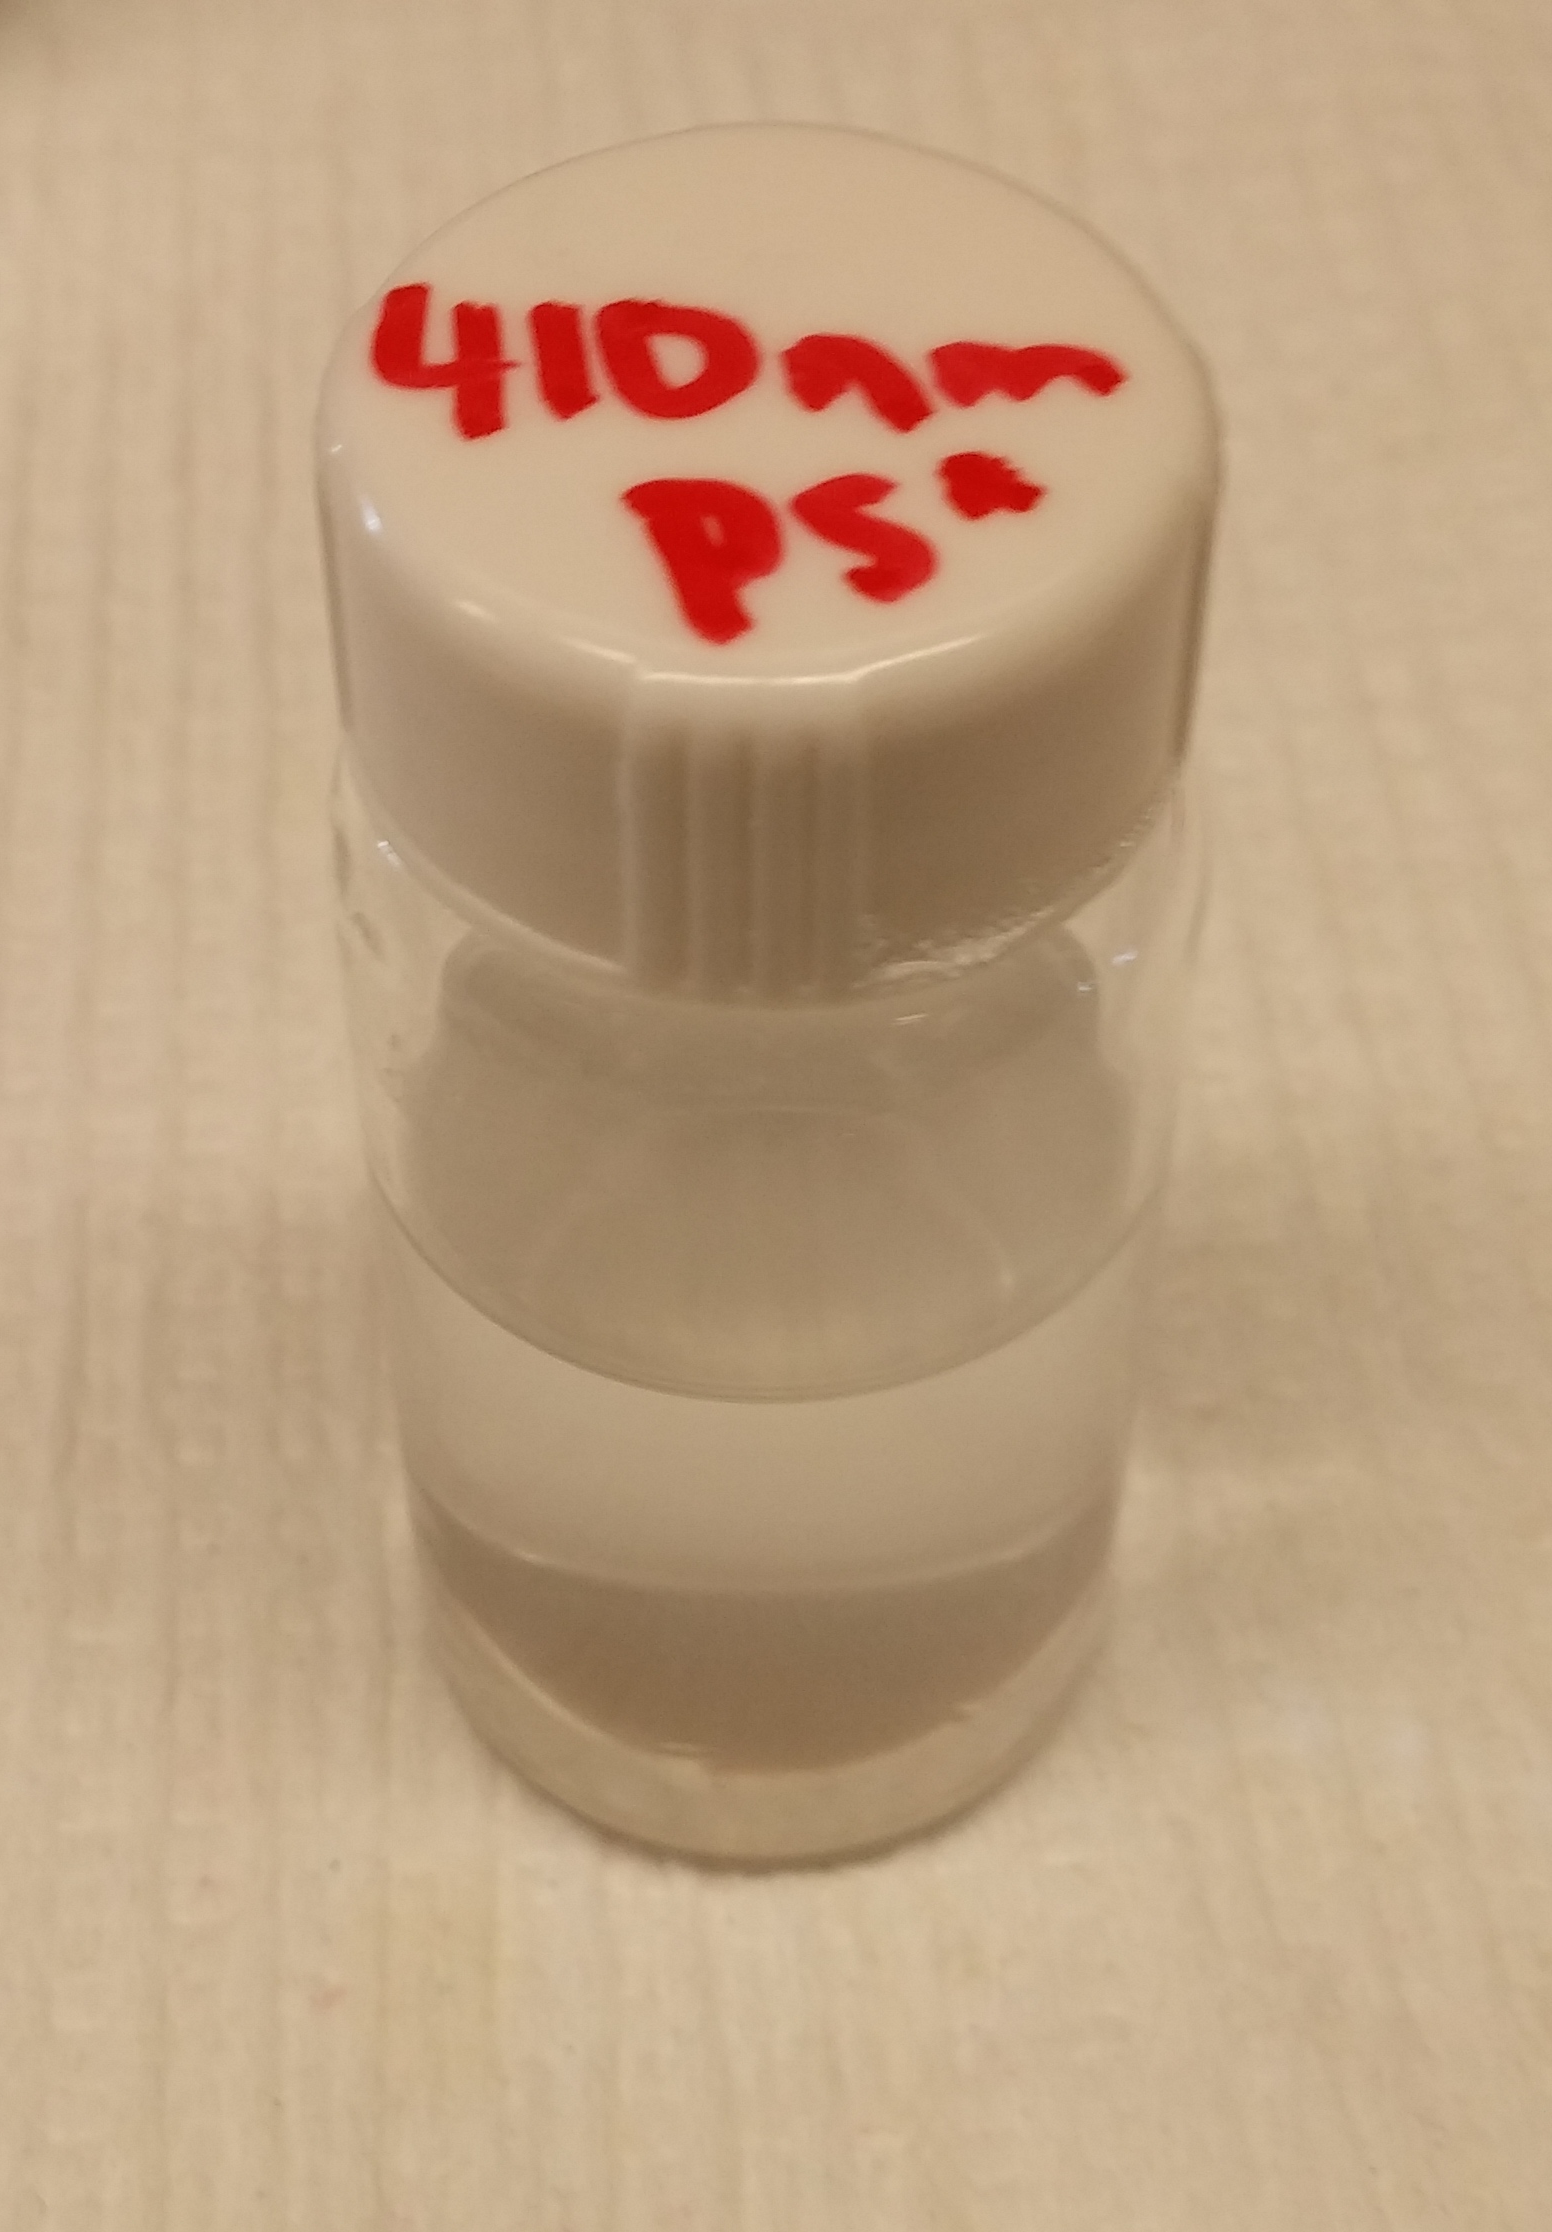
\includegraphics[width=2cm]{photo/solution.png}}
	%\end{picture}
% 	{\centering 
% 		\vspace{0.35cm}
% 		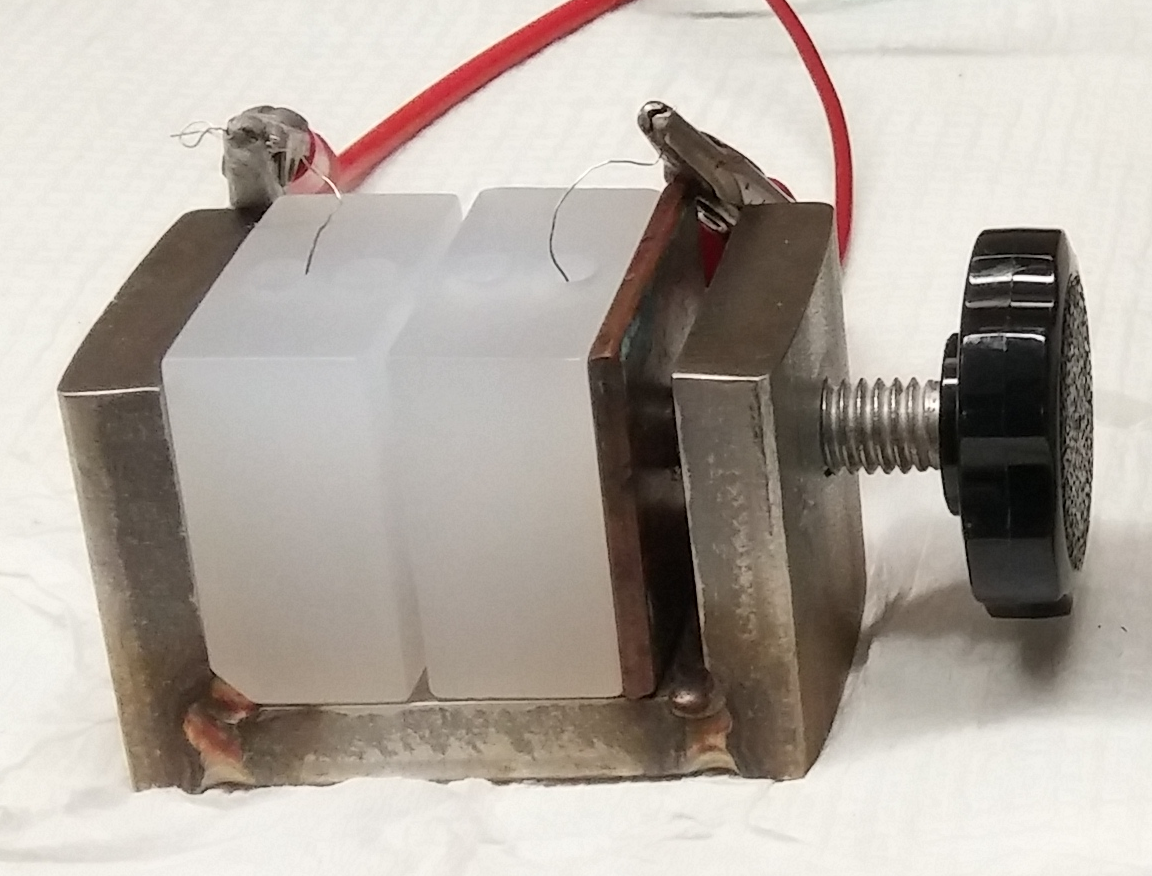
\includegraphics[width=9cm]{photo/conductivitycell.png}
% 		\newline
% 		\vspace{.35cm}
% 		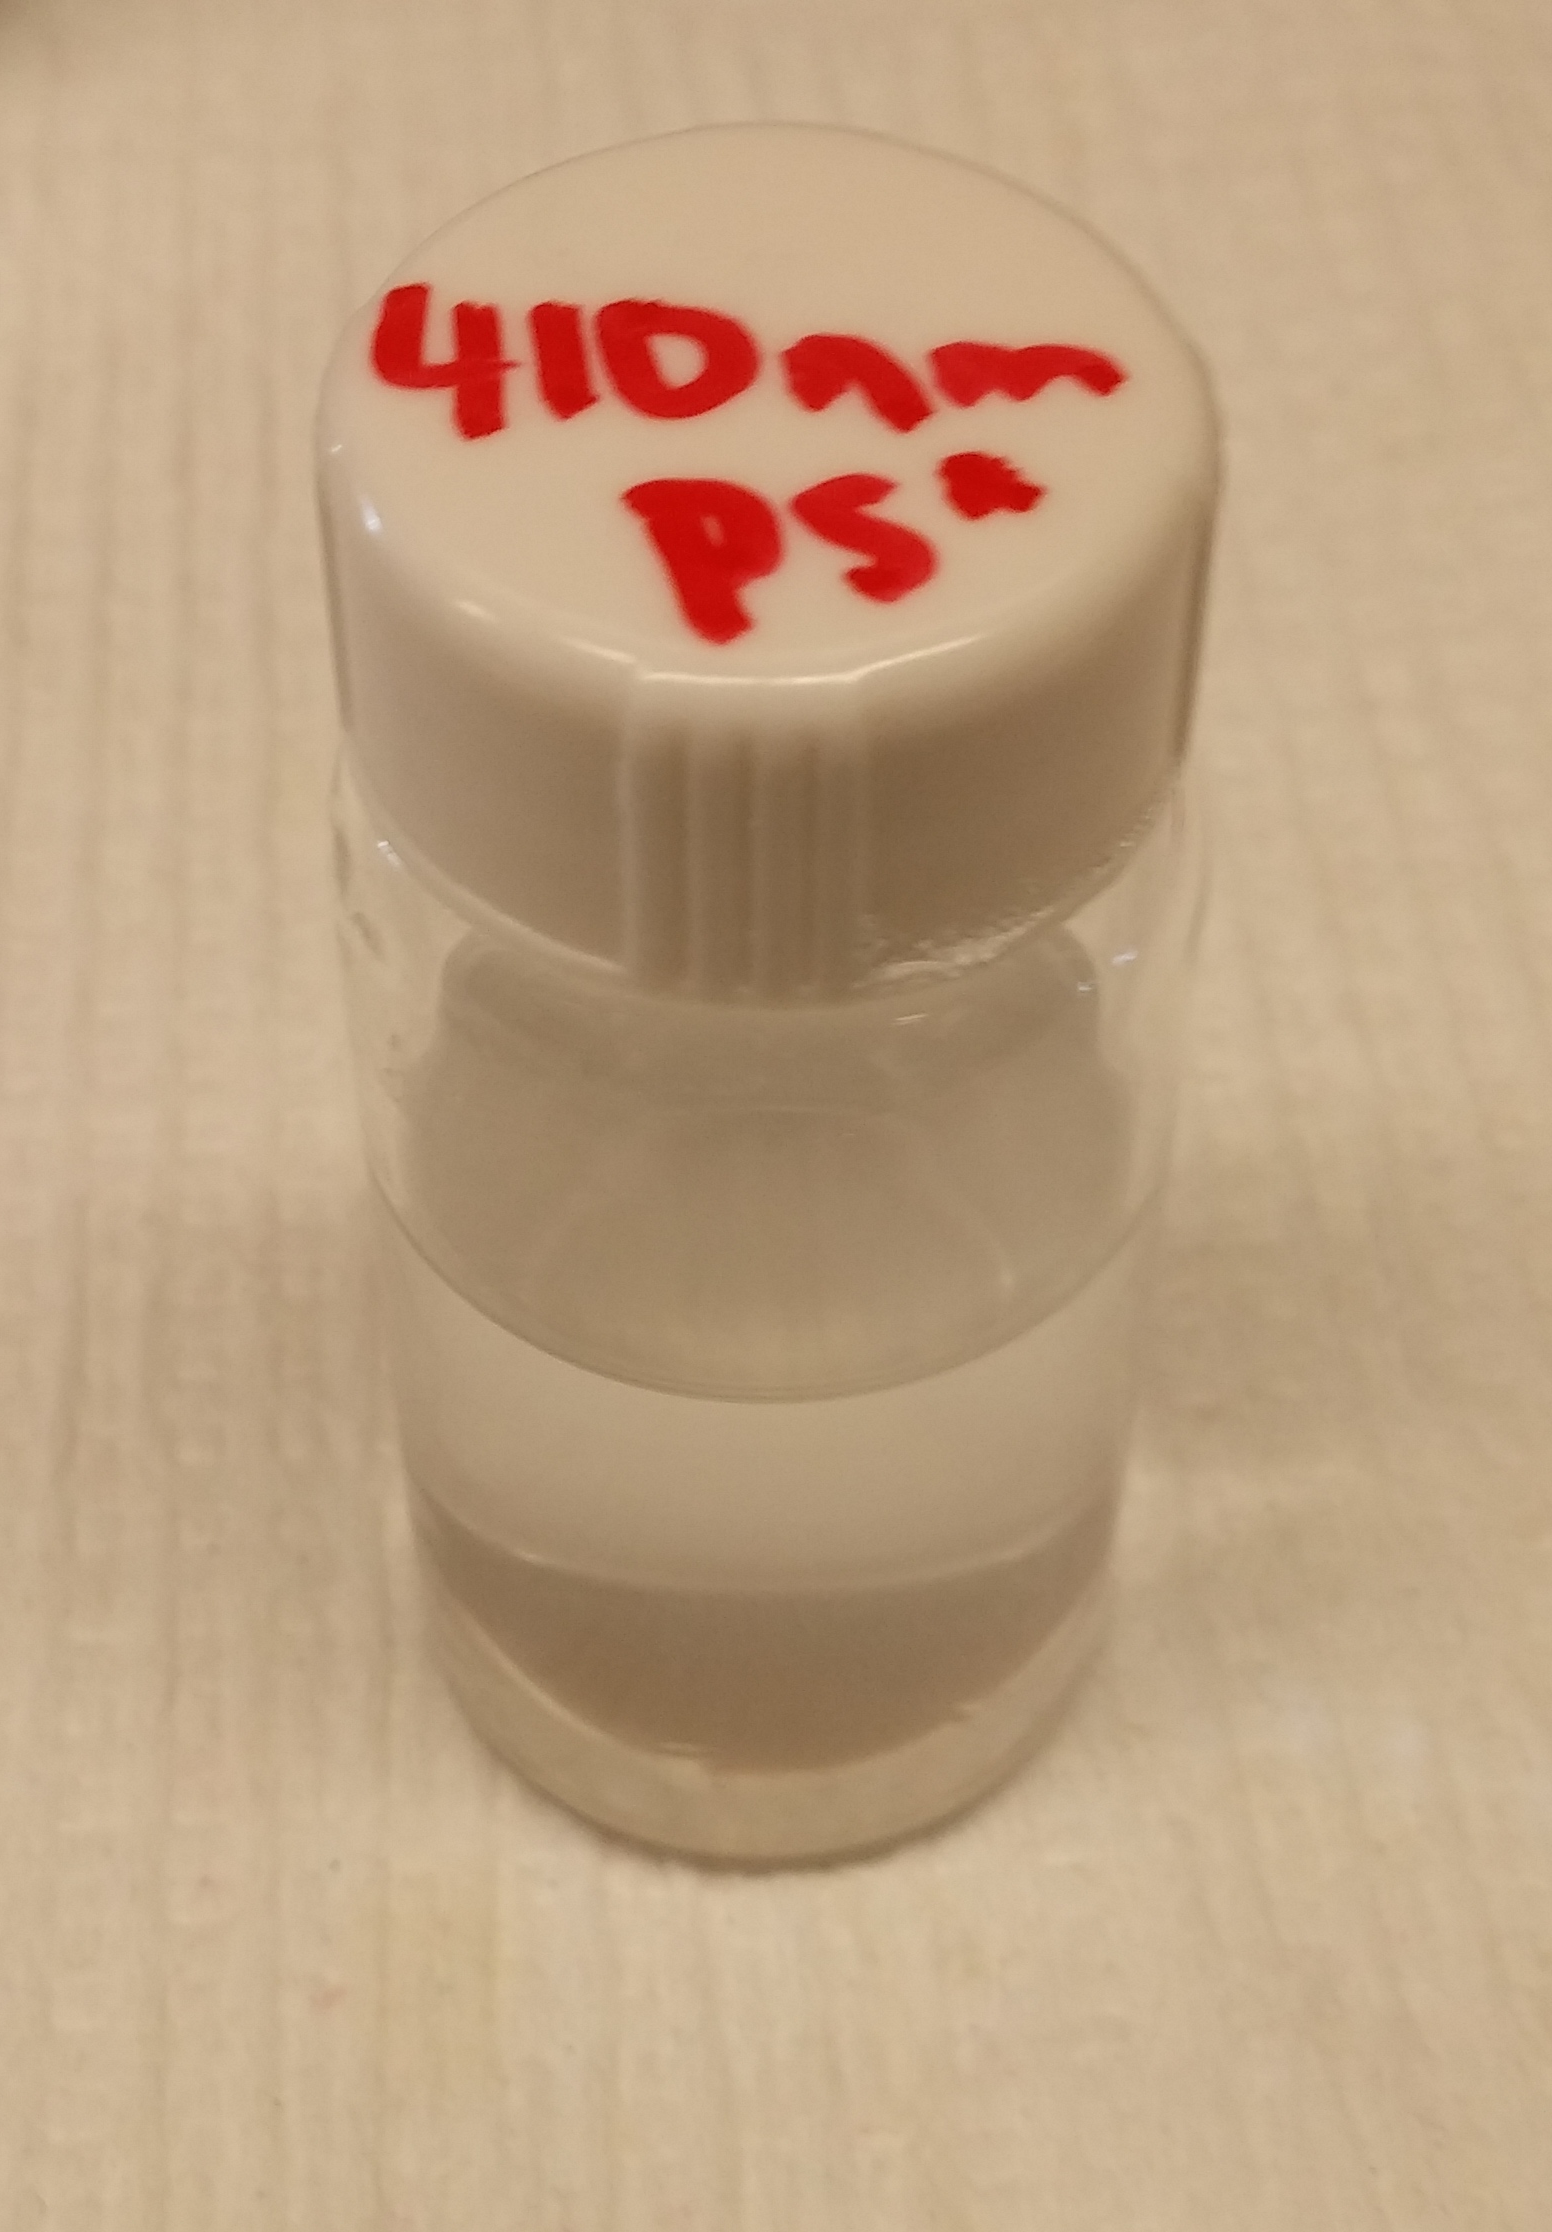
\includegraphics[width=1.5cm]{photo/solution.png}
% 		\hspace{1cm}
% 		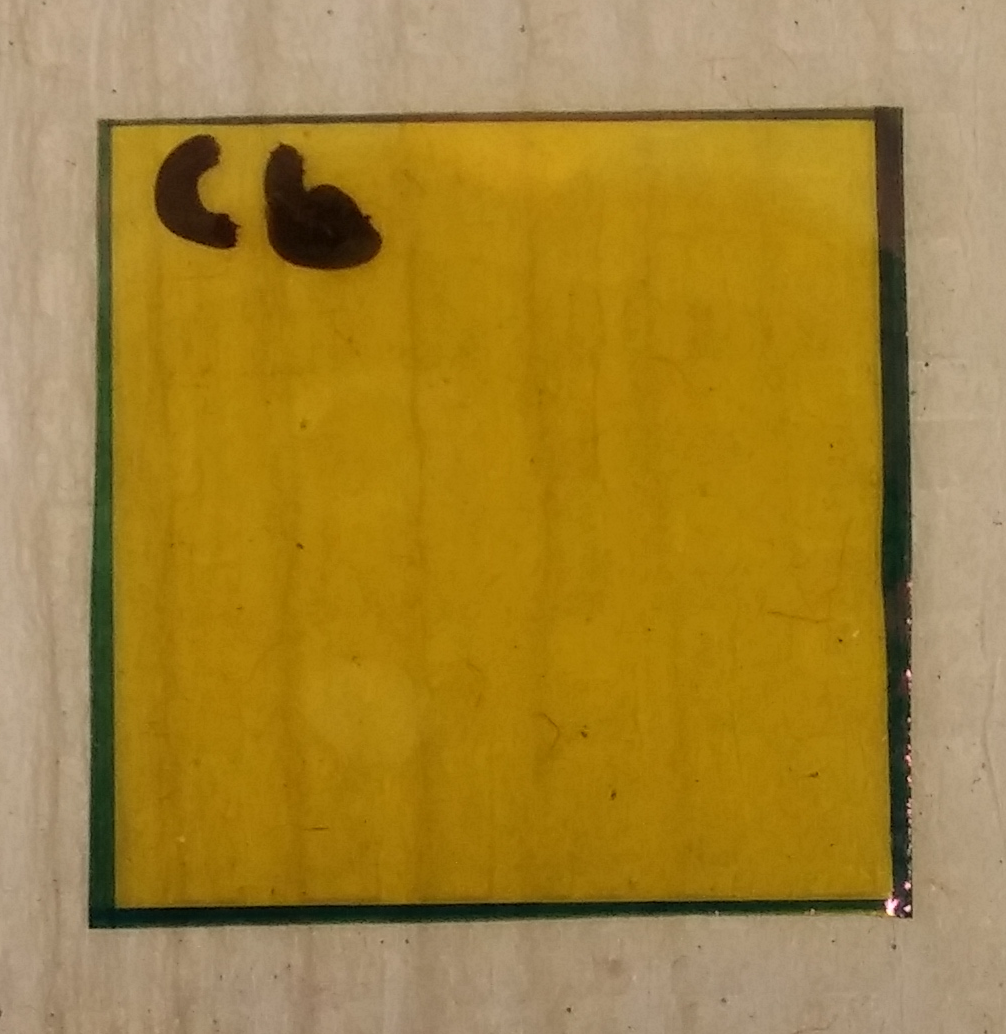
\includegraphics[width=2cm]{photo/membrane.png}
% 		\hspace{1cm}
% 		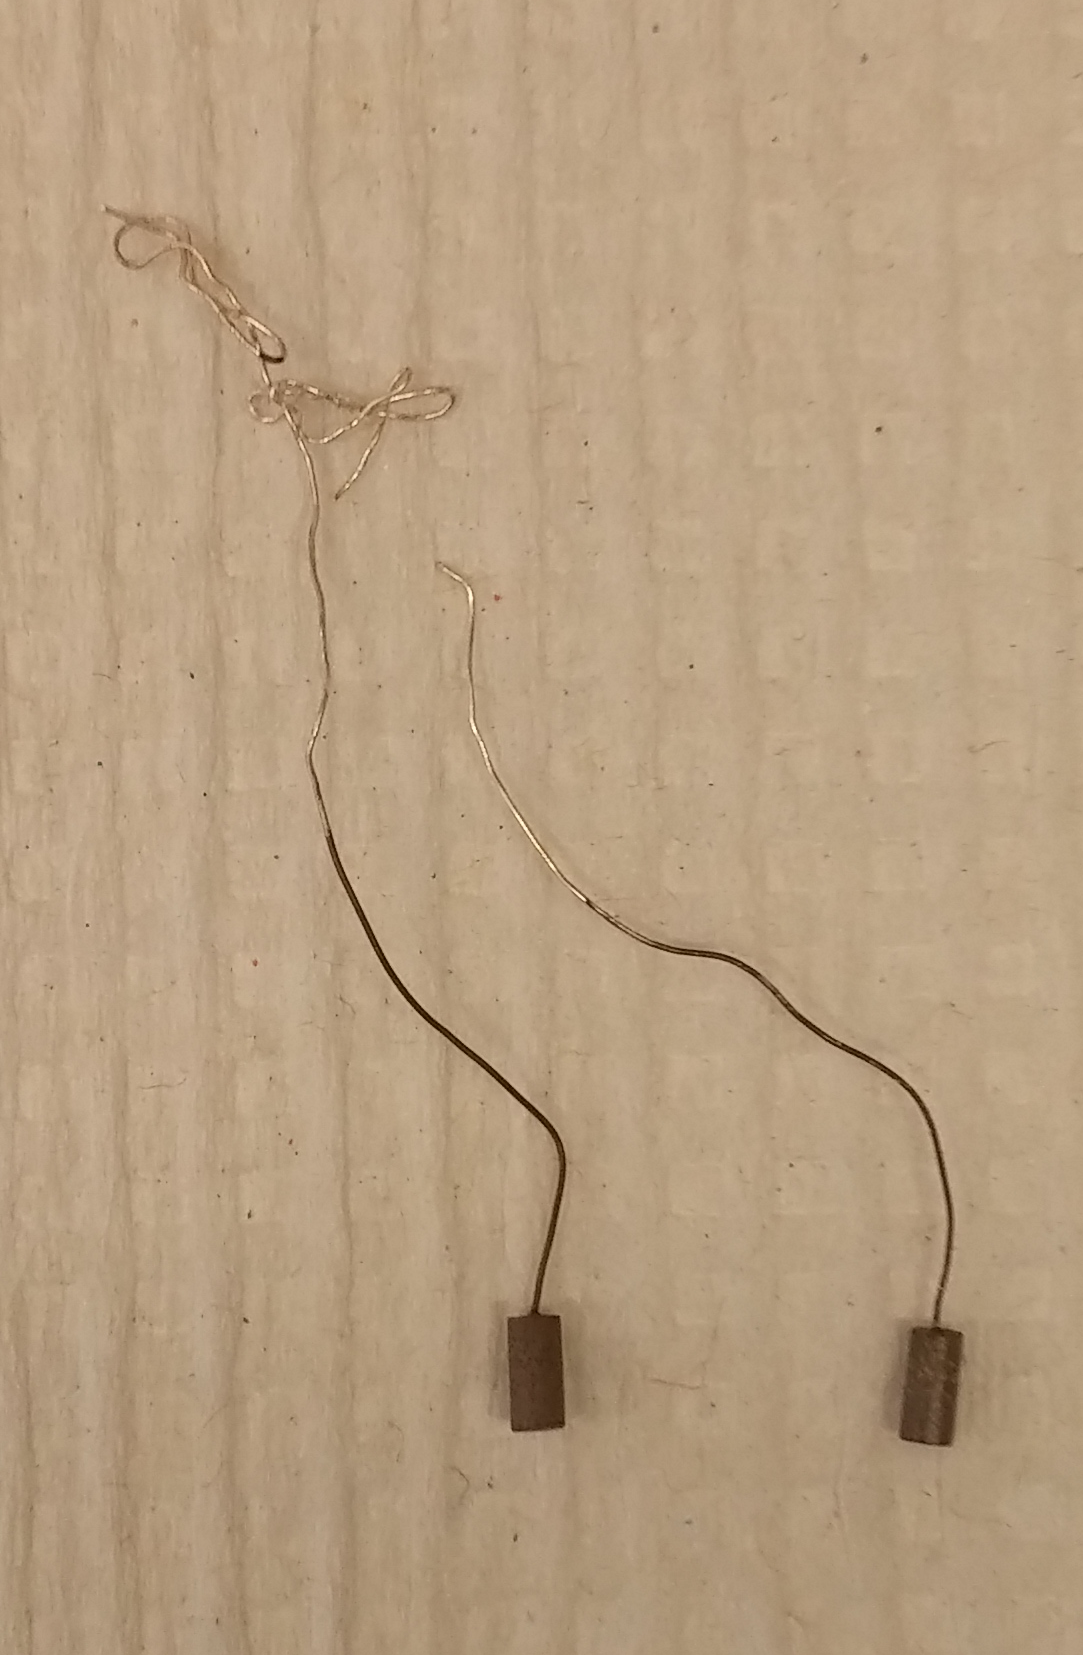
\includegraphics[width=1.5cm]{photo/electrodes.png}
% 		\hspace{1cm}
% 		\par
% 	}


	\begin{columns}[t]
		\begin{column}[T]{\paperwidth/5}
			{\centering
				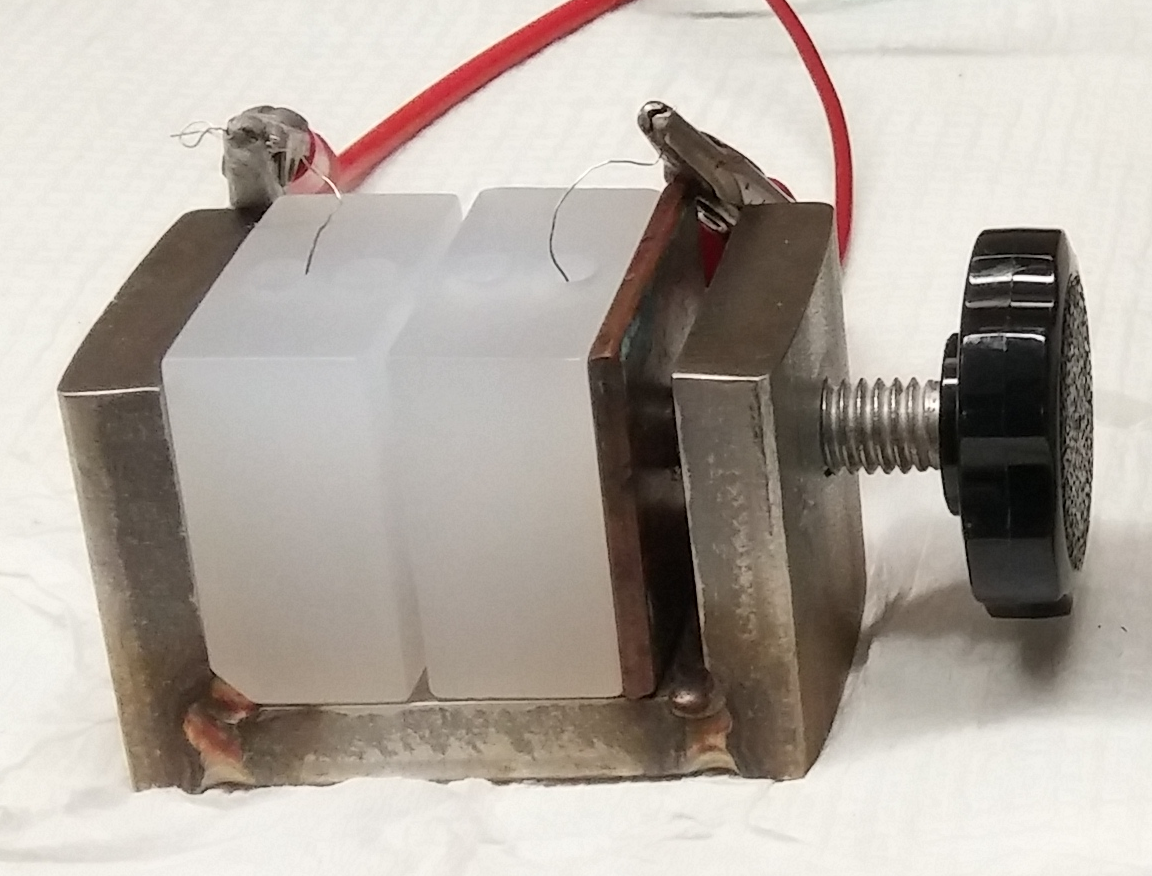
\includegraphics[height=2.25cm]{photo/conductivitycell.png} \\
				{\footnotesize Conductivity cell}
				\par
			}
		\end{column}
		
		
		\begin{column}[T]{\paperwidth/5}
			{\centering
				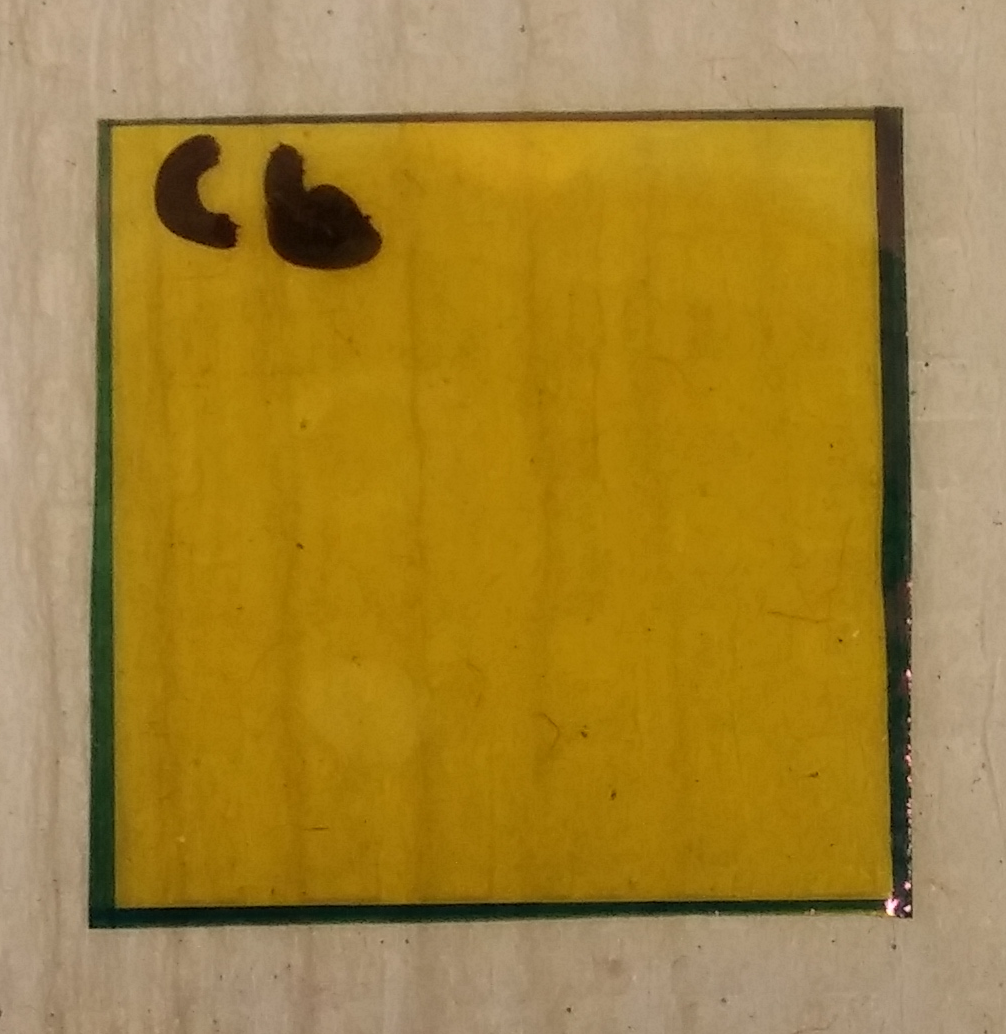
\includegraphics[height=2.25cm]{photo/membrane.png} \\
				{\footnotesize Pore membrane}
				\par
			}
		\end{column}
		
		
		
		\begin{column}[T]{\paperwidth/5}
			{\centering
				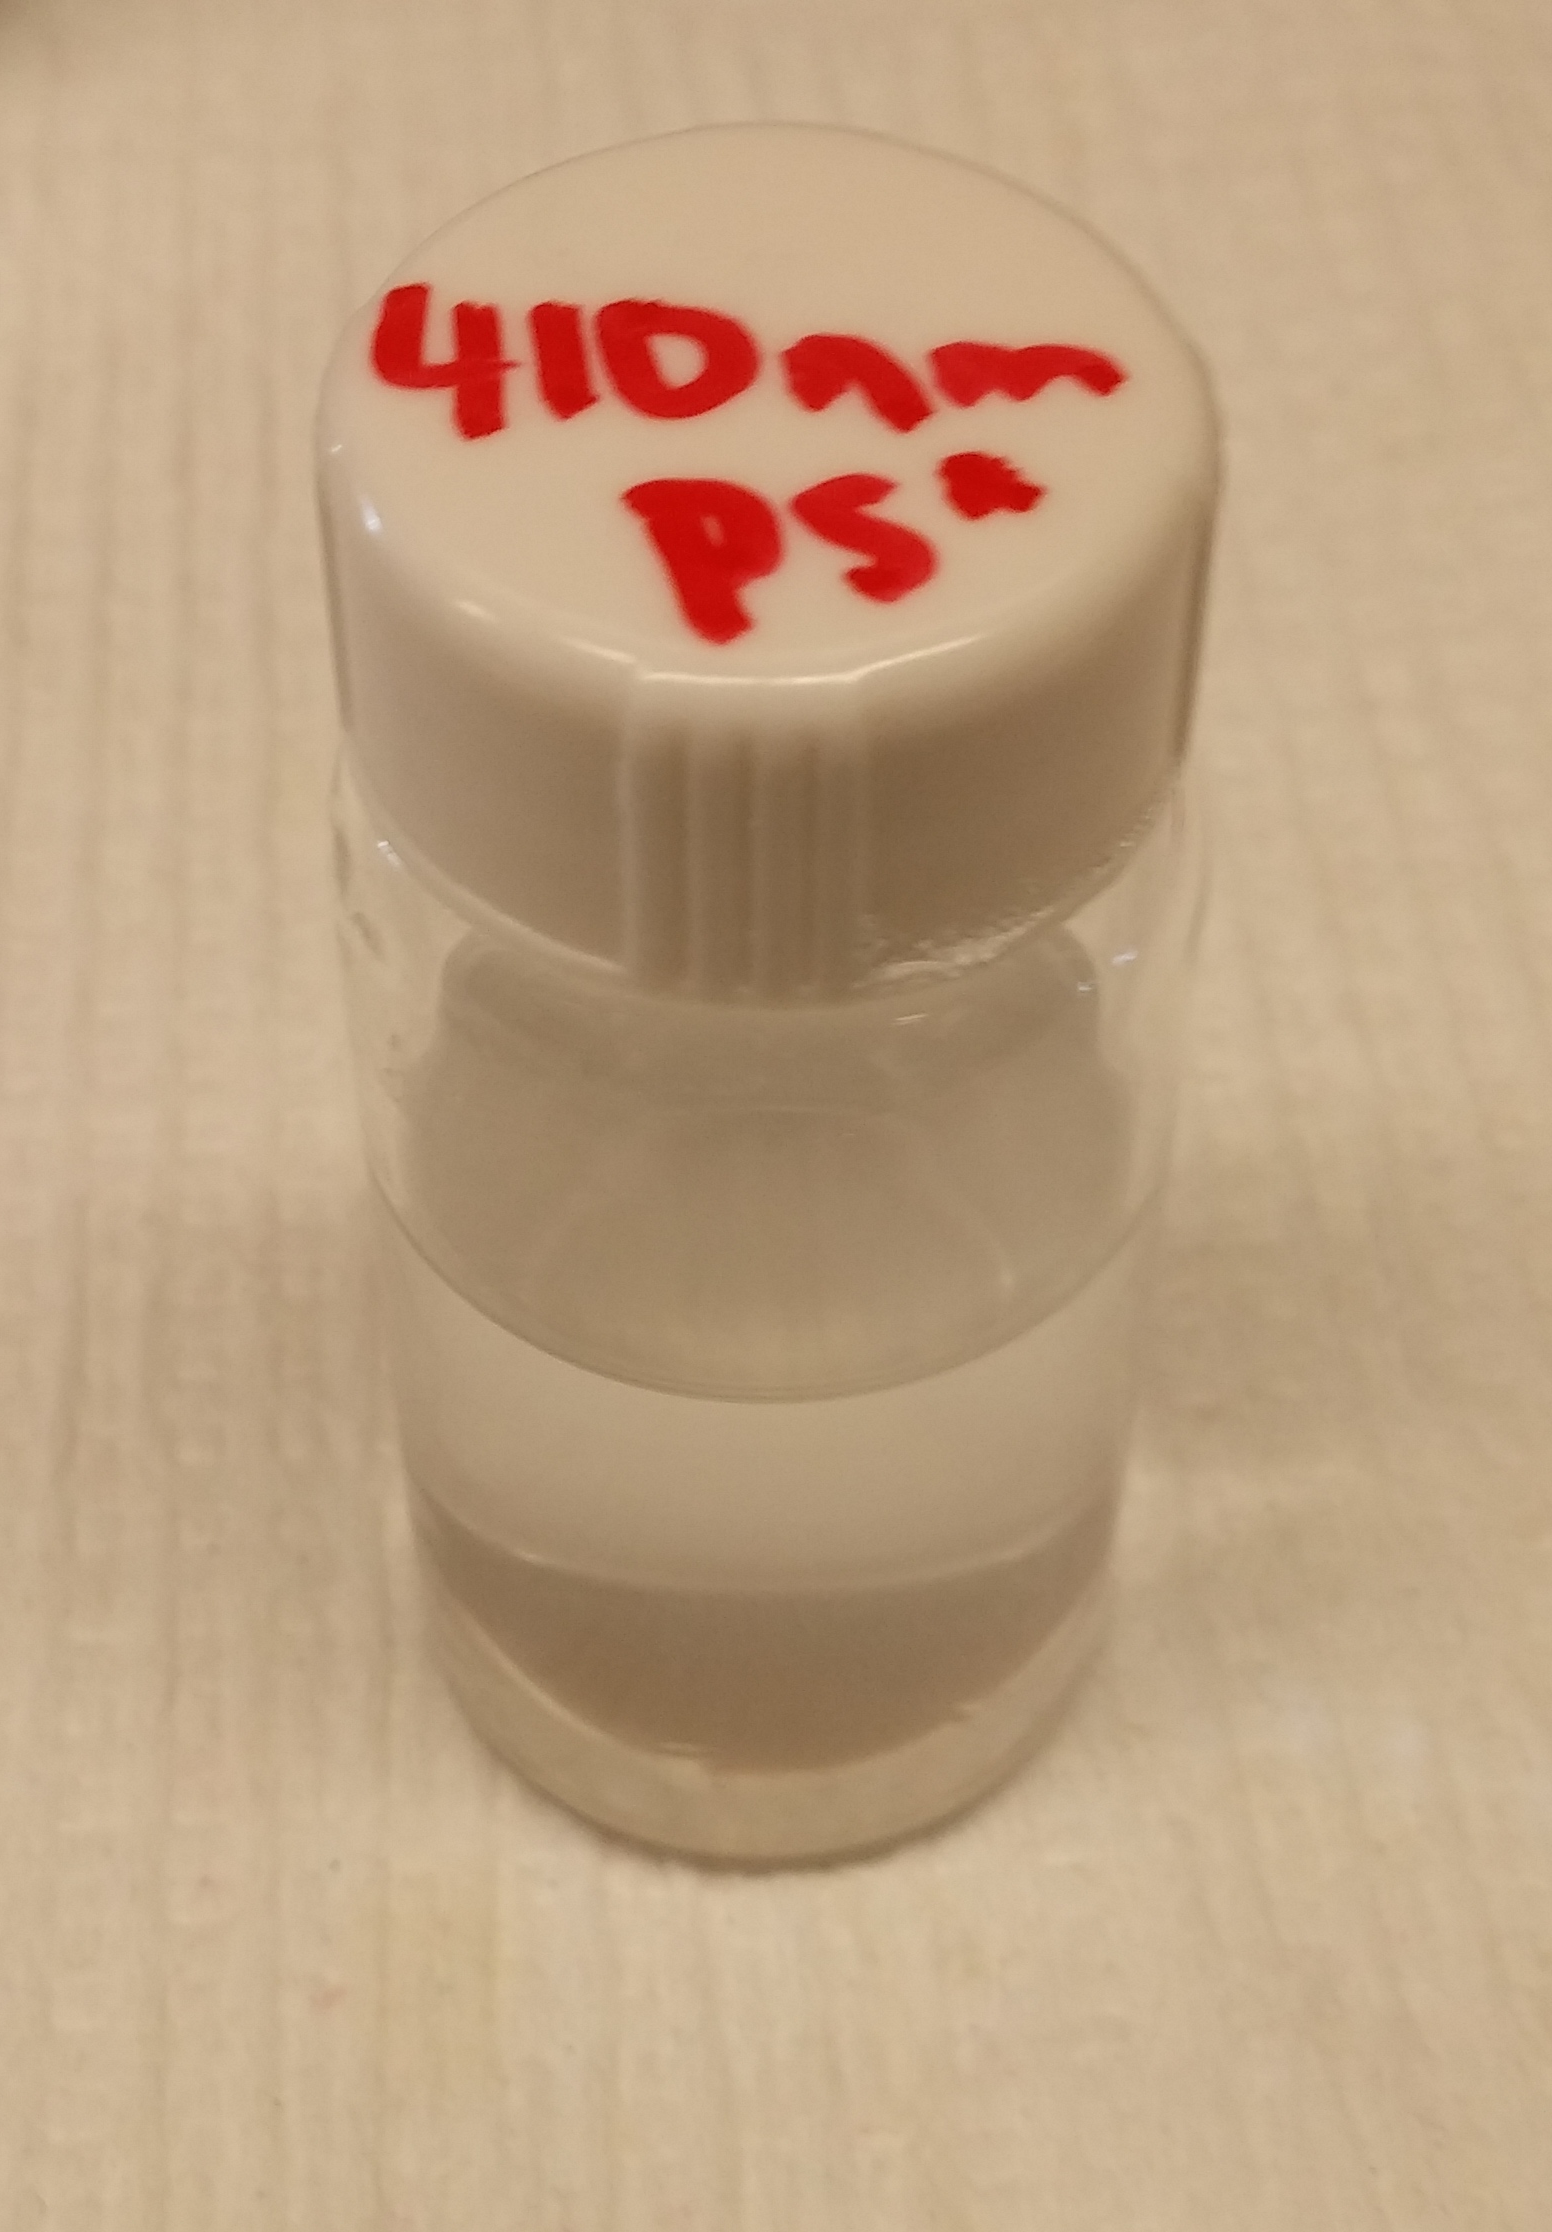
\includegraphics[height=2.25cm]{photo/solution.png} \\
				{\footnotesize Electrolyte}
				\par
			}
		\end{column}

		
		

		
		\begin{column}[T]{\paperwidth/5}
			{\centering
				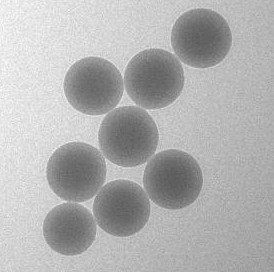
\includegraphics[height=2.25cm]{psbeads} \\
				{\footnotesize Particles}
				\par
			}
		\end{column}

	\end{columns}
	
	\vspace{1cm}
	
	\begin{columns}[t]
		\begin{column}[T]{\paperwidth/5}
			{\centering
				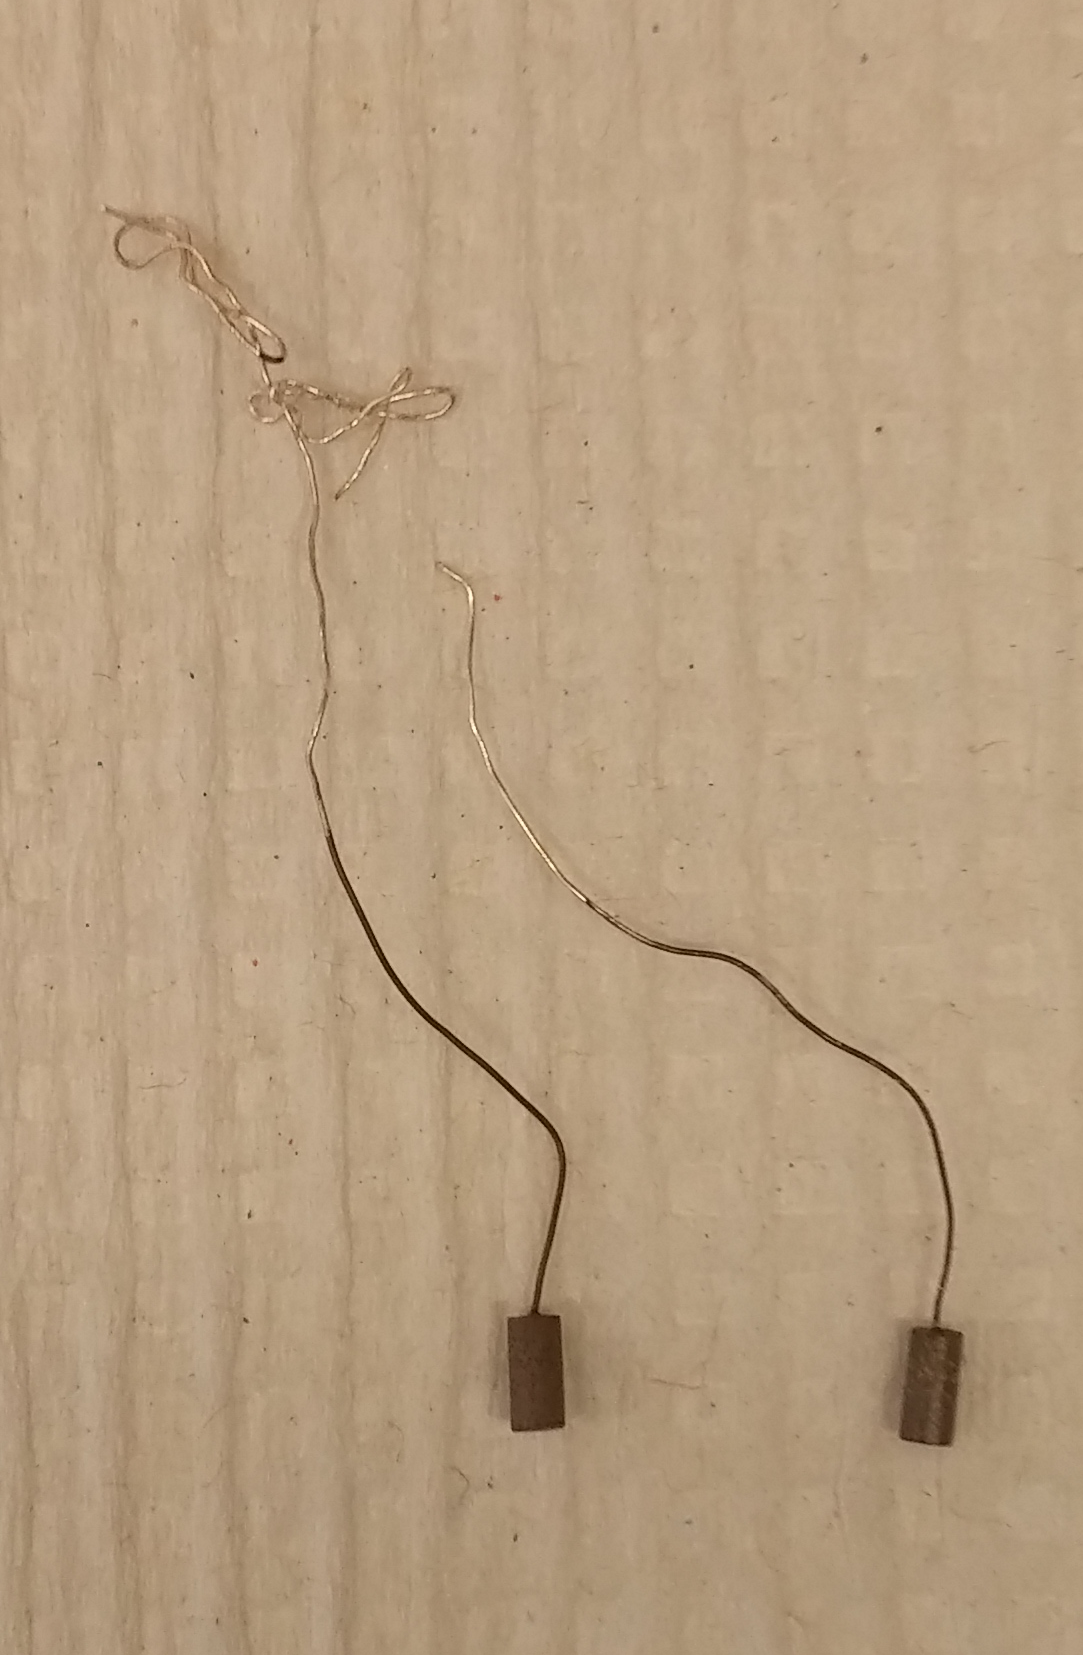
\includegraphics[height=2.25cm]{photo/electrodes.png} \\
				{\footnotesize Ag-AgCl electrodes}
				\par
			}
		\end{column}
		
		
		\begin{column}[T]{.6\paperwidth}
			{\centering
				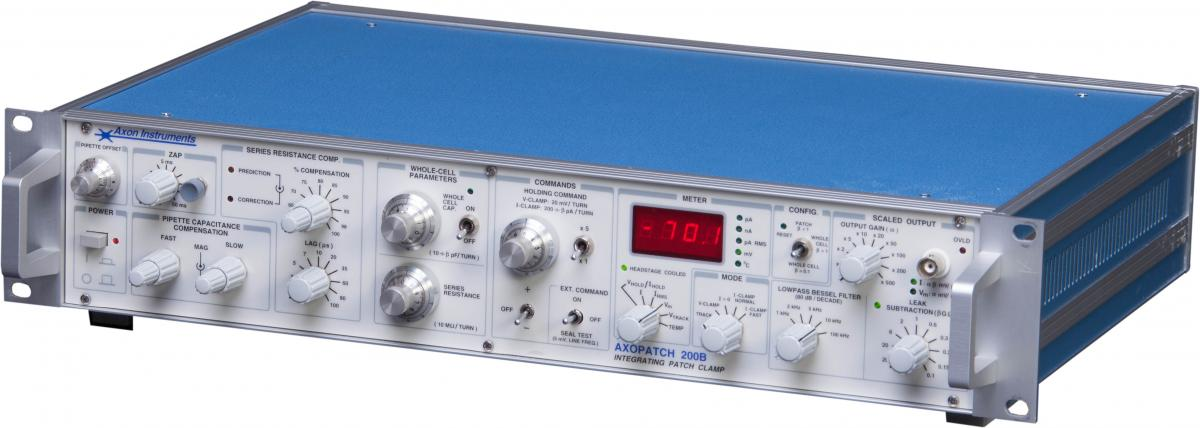
\includegraphics[height=2.25cm]{photo/axon200b} \\
				Voltage amplifier + current recorder
				\par
			}
		\end{column}
	

	\end{columns}




% 	
% 
% 
% 	\begin{center}
% 		\begin{figure}
% 		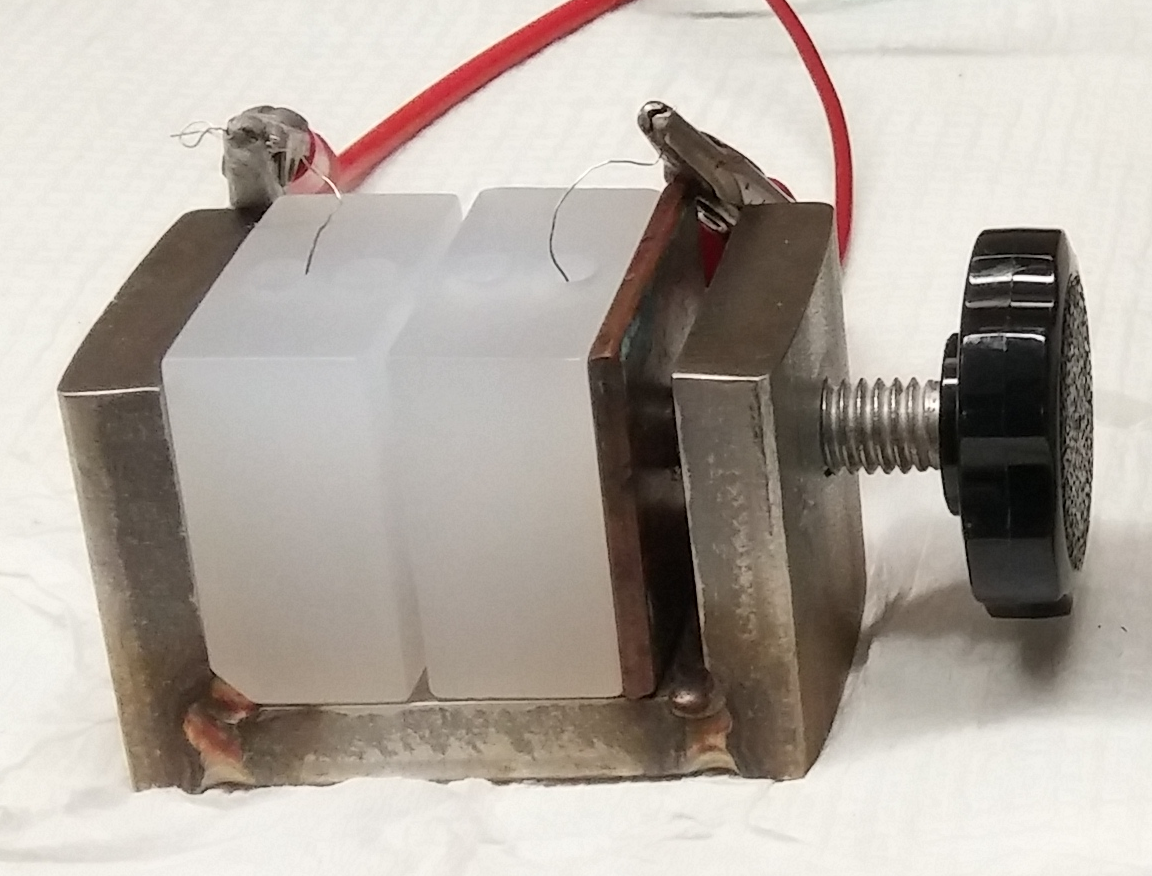
\includegraphics[height=2.25cm]{photo/conductivitycell.png}
% 		\caption{asdf}
% 		\end{figure}
% 		\hspace{.35cm}
%  		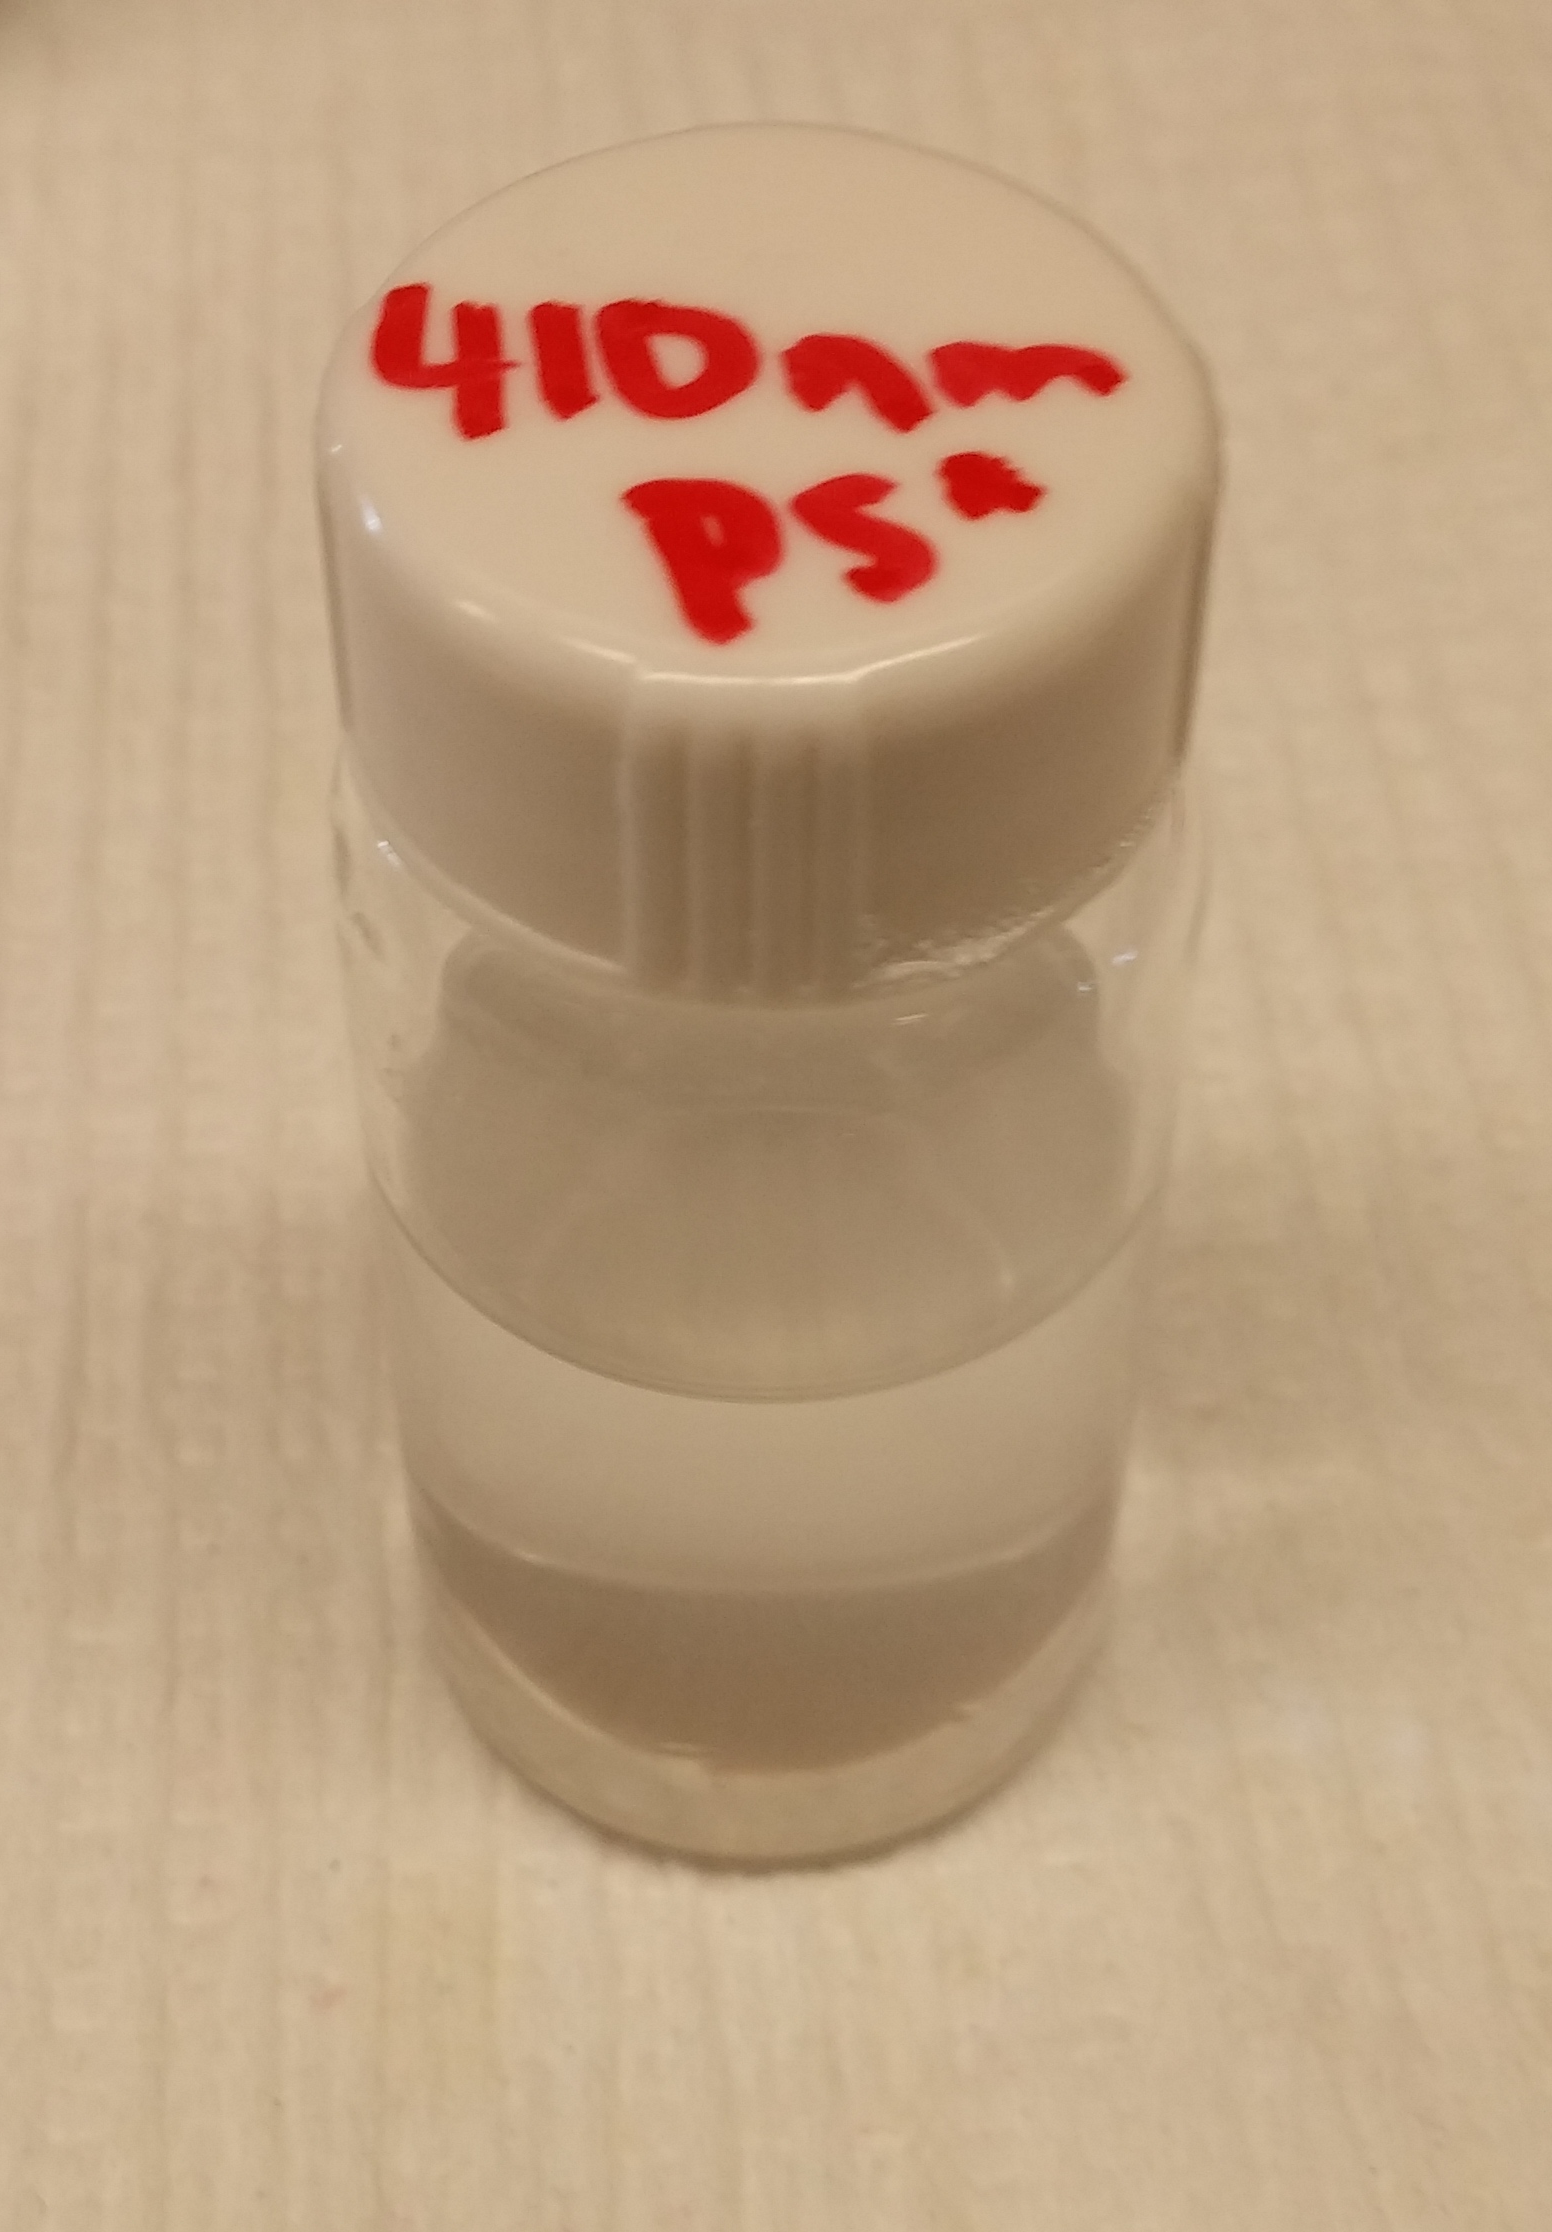
\includegraphics[height=2.25cm]{photo/solution.png}
%  		\hspace{.35cm}
%  		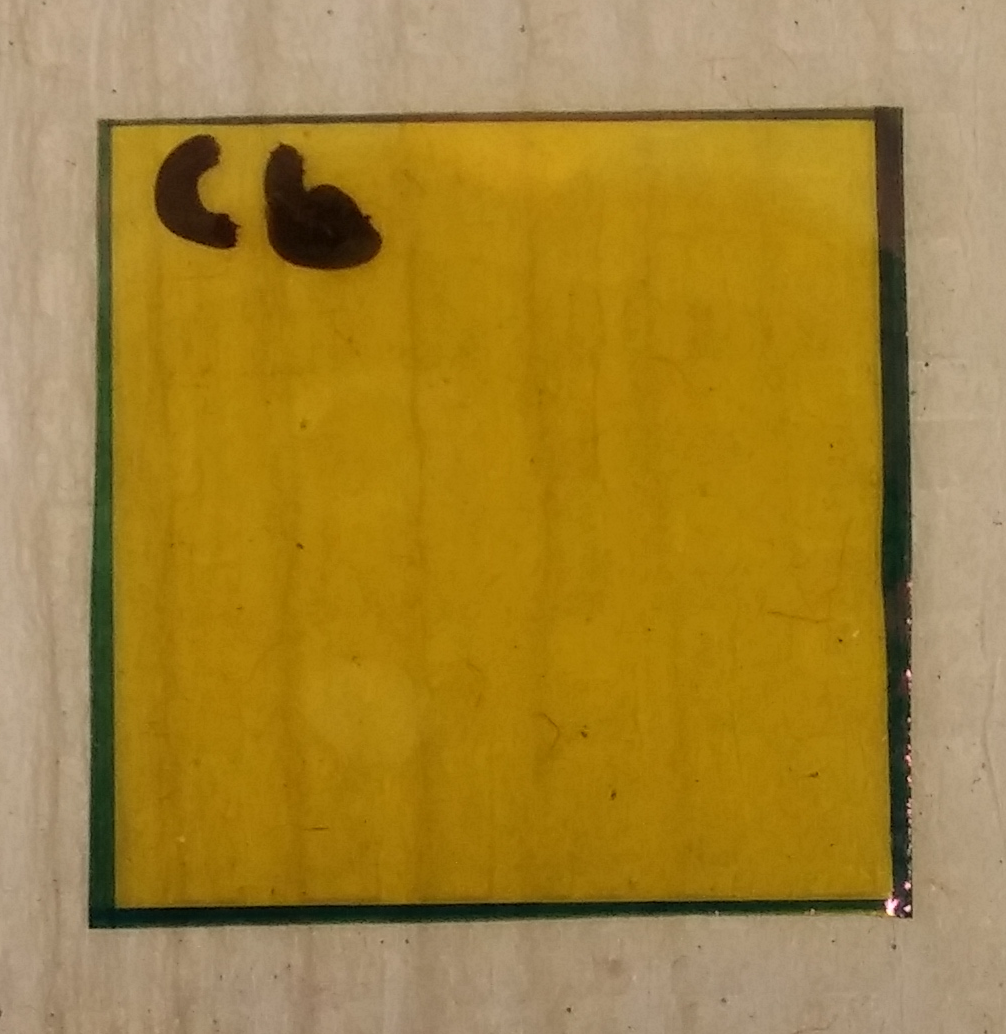
\includegraphics[height=2.25cm]{photo/membrane.png}
%  		\hspace{.35cm}
%  		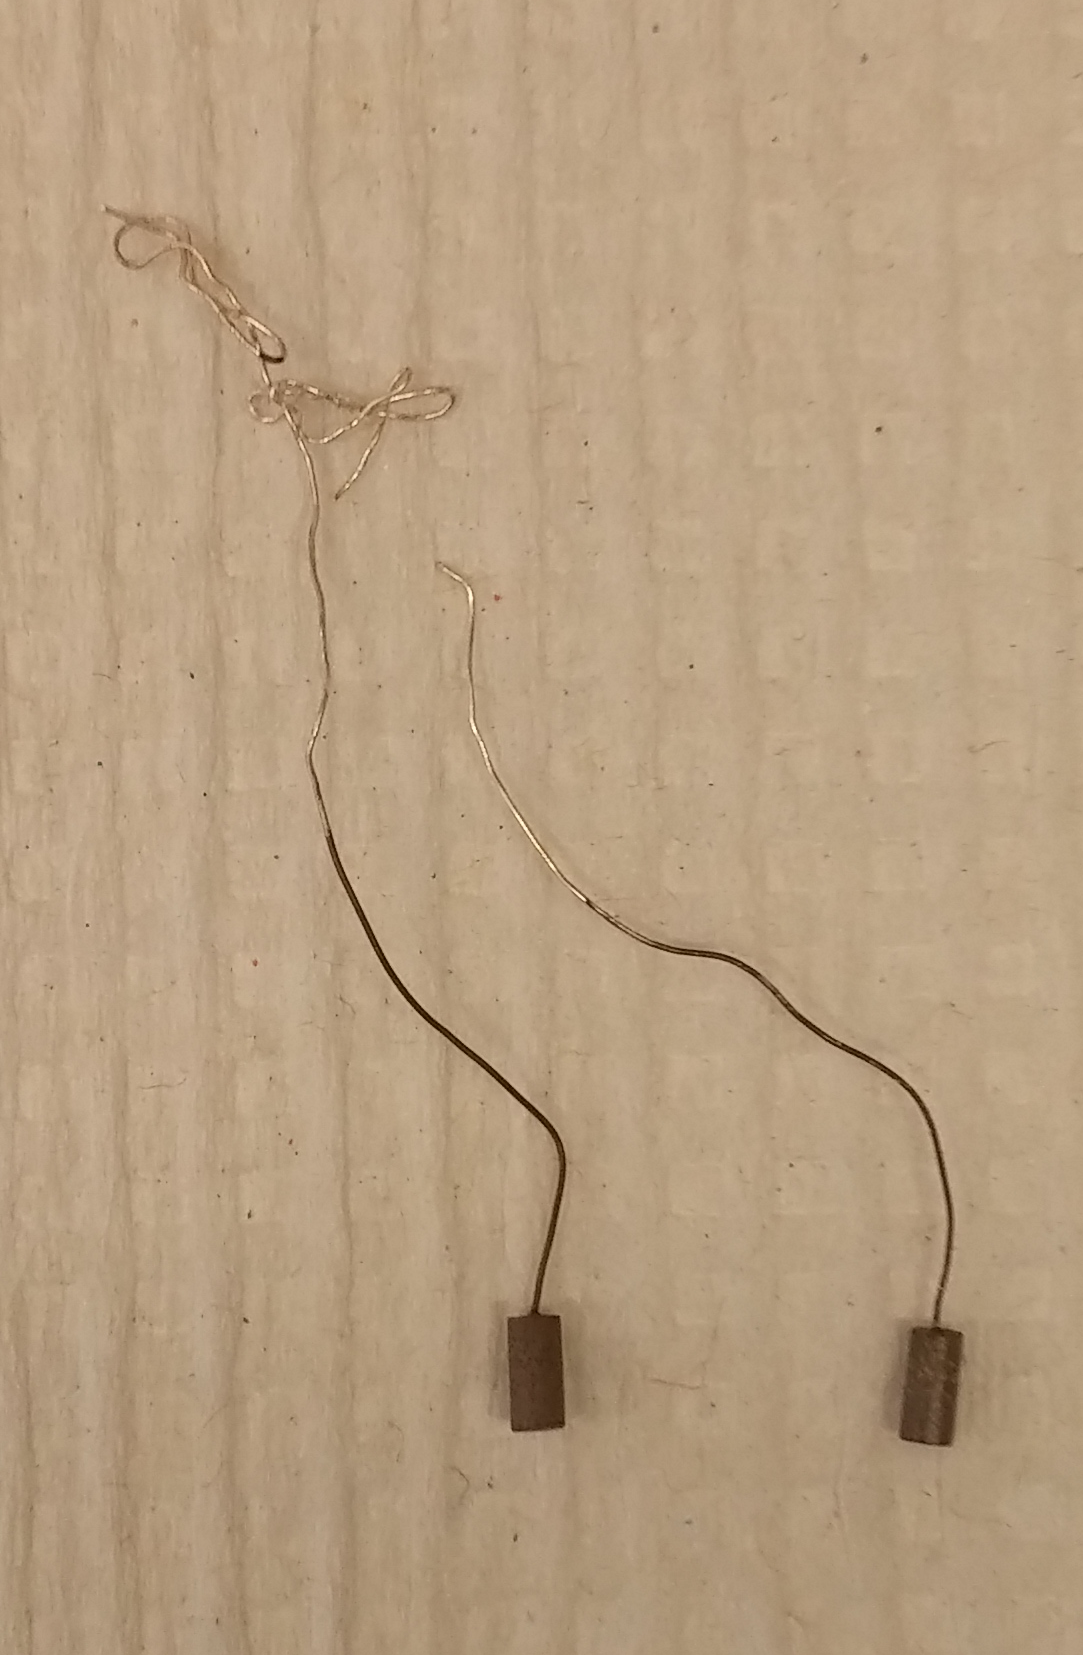
\includegraphics[height=2.25cm]{photo/electrodes.png}
%  		\hspace{.35cm}
% 	\end{center}

\end{frame}

%%%%%%%%%%%%%%%%%%%%%%%%%%%%%%%%%%%%%%%%%%%%%%%%%%%%%%%%%%%%%%%%%%%%%%%%%%%%%%%%%%%%%%%%%%%%%%%%%%%%%%%%%%%%%%%%%%%%%%%%%%%%
% Resistive pulse background---electrostatic boundary conditions
%%%%%%%%%%%%%%%%%%%%%%%%%%%%%%%%%%%%%%%%%%%%%%%%%%%%%%%%%%%%%%%%%%%%%%%%%%%%%%%%%%%%%%%%%%%%%%%%%%%%%%%%%%%%%%%%%%%%%%%%%%%%

\begin{frame}[c]{Resistive pulse sensing}
	{\centering
		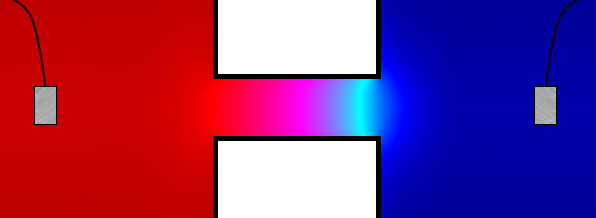
\includegraphics[width=0.9\paperwidth]{comsol/voltage.png}
		\par
	}
\end{frame}

%%%%%%%%%%%%%%%%%%%%%%%%%%%%%%%%%%%%%%%%%%%%%%%%%%%%%%%%%%%%%%%%%%%%%%%%%%%%%%%%%%%%%%%%%%%%%%%%%%%%%%%%%%%%%%%%%%%%%%%%%%%%
% Resistive pulse background---electrostatic boundary conditions
%%%%%%%%%%%%%%%%%%%%%%%%%%%%%%%%%%%%%%%%%%%%%%%%%%%%%%%%%%%%%%%%%%%%%%%%%%%%%%%%%%%%%%%%%%%%%%%%%%%%%%%%%%%%%%%%%%%%%%%%%%%%

\begin{frame}[c]{Resistive pulse sensing---electrostatic boundary conditions}
	{\centering
		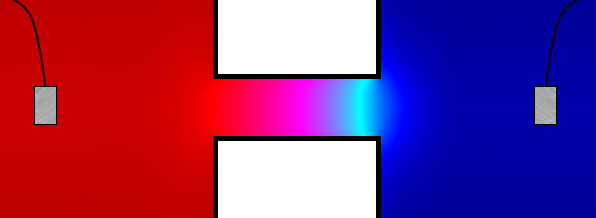
\includegraphics[width=0.9\paperwidth]{comsol/voltage.png}
		\par
	}
\end{frame}


%%%%%%%%%%%%%%%%%%%%%%%%%%%%%%%%%%%%%%%%%%%%%%%%%%%%%%%%%%%%%%%%%%%%%%%%%%%%%%%%%%%%%%%%%%%%%%%%%%%%%%%%%%%%%%%%%%%%%%%%%%%%
% Resistive pulse background---ion transport
%%%%%%%%%%%%%%%%%%%%%%%%%%%%%%%%%%%%%%%%%%%%%%%%%%%%%%%%%%%%%%%%%%%%%%%%%%%%%%%%%%%%%%%%%%%%%%%%%%%%%%%%%%%%%%%%%%%%%%%%%%%%

\tikzset{cross/.style={cross out, draw=black, minimum size=2*(#1-\pgflinewidth), inner sep=0pt, outer sep=0pt},
%default radius will be 1pt. 
cross/.default={1pt}}



\begin{frame}[c]{Resistive pulse sensing---ion transport}
	\begin{itemize}
		\item Ion transport is driven by \textbf{diffusion}, \textbf{convection}, and \textbf{electric migration}
		\item \underline{Diffusion}: Average flow of ions from high to low concentration
		\item \underline{Convection}: Ions move with the fluid/solvent
		\item \underline{Electrical migration}: Ions move in electric field
	\end{itemize}
	\only<1>{
		$$ \vec{J}_{i}=\underbrace{z_{i}eD_{i}\nabla c_{i}}_{\mathrm{diffusion}}+\overbrace{z_{i}ec_{i}\vec{u}}^{\mathrm{convection}}+\underbrace{z_{i}ec_{i}\mu_{i}\vec{E}}_{\mathrm{migration}} $$
	}
	\only<2>{
		$$ \vec{J}_{i}=\underbrace{\xcancel{z_{i}eD_{i}\nabla c_{i}}}_{\mathrm{diffusion}}+\overbrace{\xcancel{z_{i}ec_{i}\vec{u}}}^{\mathrm{convection}}+\underbrace{z_{i}ec_{i}\mu_{i}\vec{E}}_{\mathrm{migration}} $$
	}
	
	$$ I=\sum_{i}\iint_{S}\vec{J_{i}}\cdot \hat{n}dS $$
	
	% xs over two terms in equation
	\onslide<2>{
		\begin{tikzpicture}[]
			\draw(300,25) node[cross=10pt,red] {};
			\draw(1,0) node[cross=10pt,red] {};
		\end{tikzpicture}
	}

\end{frame}




%%%%%%%%%%%%%%%%%%%%%%%%%%%%%%%%%%%%%%%%%%%%%%%%%%%%%%%%%%%%%%%%%%%%%%%%%%%%%%%%%%%%%%%%%%%%%%%%%%%%%%%%%%%%%%%%%%%%%%%%%%%%
% Rods title slide
%%%%%%%%%%%%%%%%%%%%%%%%%%%%%%%%%%%%%%%%%%%%%%%%%%%%%%%%%%%%%%%%%%%%%%%%%%%%%%%%%%%%%%%%%%%%%%%%%%%%%%%%%%%%%%%%%%%%%%%%%%%%


\begin{frame}[c]{}
	\begin{center}
		\textbf{Resistive pulse sensing of high-aspect ratio particles}
	\end{center}
\end{frame}




%%%%%%%%%%%%%%%%%%%%%%%%%%%%%%%%%%%%%%%%%%%%%%%%%%%%%%%%%%%%%%%%%%%%%%%%%%%%%%%%%%%%%%%%%%%%%%%%%%%%%%%%%%%%%%%%%%%%%%%%%%%%
% Rods motivation slide
%%%%%%%%%%%%%%%%%%%%%%%%%%%%%%%%%%%%%%%%%%%%%%%%%%%%%%%%%%%%%%%%%%%%%%%%%%%%%%%%%%%%%%%%%%%%%%%%%%%%%%%%%%%%%%%%%%%%%%%%%%%%


\begin{frame}[c]{High-aspect ratio resistive pulse sensing---motivation}
	\begin{itemize}
		\item Aspherical particles are ubiquitous in biology---e.g., viruses, bacteria 
		\item RP sensing allows volume determination
		\item Can we extend RP to measure length?
		\item How would we do so?
	\end{itemize}
	{\centering
		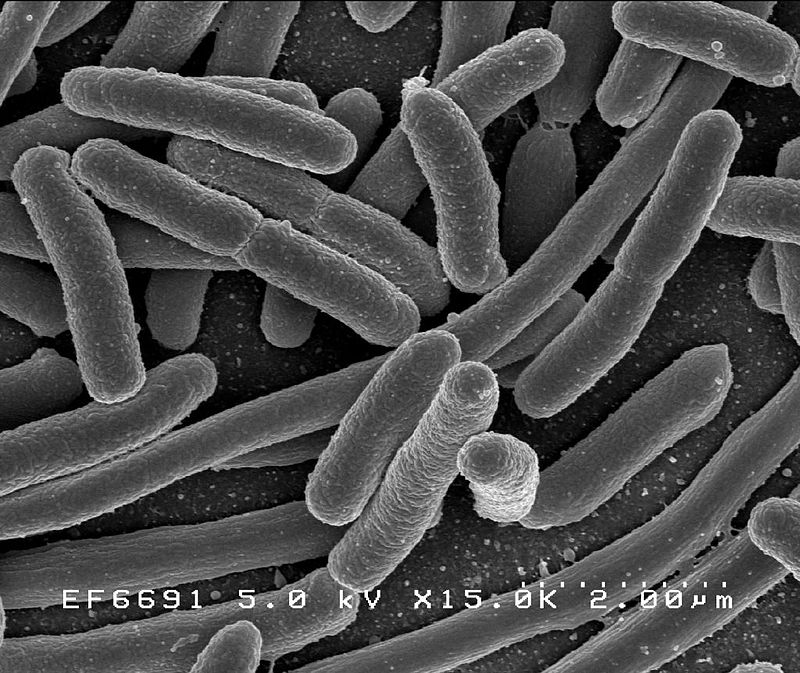
\includegraphics[height=3cm]{ecoli}
		\hspace{1cm}
		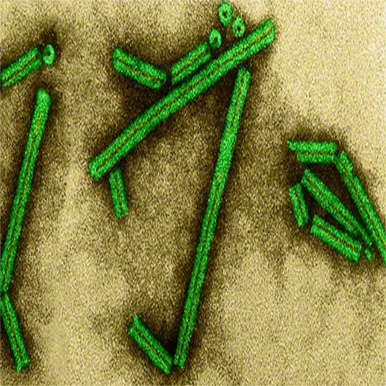
\includegraphics[height=3cm]{tobaccomosaicvirus}
		\par
	}
\end{frame}




%%%%%%%%%%%%%%%%%%%%%%%%%%%%%%%%%%%%%%%%%%%%%%%%%%%%%%%%%%%%%%%%%%%%%%%%%%%%%%%%%%%%%%%%%%%%%%%%%%%%%%%%%%%%%%%%%%%%%%%%%%%%
% Length convolution explanation
%%%%%%%%%%%%%%%%%%%%%%%%%%%%%%%%%%%%%%%%%%%%%%%%%%%%%%%%%%%%%%%%%%%%%%%%%%%%%%%%%%%%%%%%%%%%%%%%%%%%%%%%%%%%%%%%%%%%%%%%%%%%

\begin{frame}[c]{Resistive pulse in non-constant width pores}
	\begin{itemize}
		\item Change in resistance of pore is approximately
	\end{itemize}
	$$ \Delta R\left(z'\right)=\frac{\rho}{\pi}\int_{z=z'}^{z=z'+l_{p}}\frac{dz}{r_{P}^{2}\left(z\right)-s_{p}^{2}\left(z\right)} $$
	\begin{itemize}
		\item RP amplitude is a function of the pore geometry \textbf{local to the particle's position}
		\item Particles map the interior of the pore during translocation with their RP signal!
	\end{itemize}
	
	{\centering
		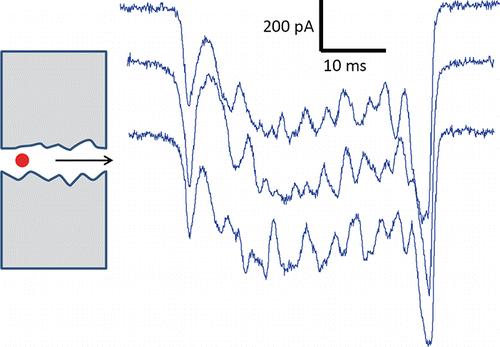
\includegraphics[width=2in]{particlesreveal.png} \\
		\par
	}
	
	
	
\end{frame}


%%%%%%%%%%%%%%%%%%%%%%%%%%%%%%%%%%%%%%%%%%%%%%%%%%%%%%%%%%%%%%%%%%%%%%%%%%%%%%%%%%%%%%%%%%%%%%%%%%%%%%%%%%%%%%%%%%%%%%%%%%%%
% Length convolution explanation
%%%%%%%%%%%%%%%%%%%%%%%%%%%%%%%%%%%%%%%%%%%%%%%%%%%%%%%%%%%%%%%%%%%%%%%%%%%%%%%%%%%%%%%%%%%%%%%%%%%%%%%%%%%%%%%%%%%%%%%%%%%%

\begin{frame}[c]{Resistive pulse in non-constant width pores}
	\begin{itemize}
		\item For particles with length shorter than characteristic length of changes in pore size, the interior is mapped with high resolution
		\item Long particles map pore interiors with low resolution because their lengths extend along multiple features
	\end{itemize}
	
	{\centering
		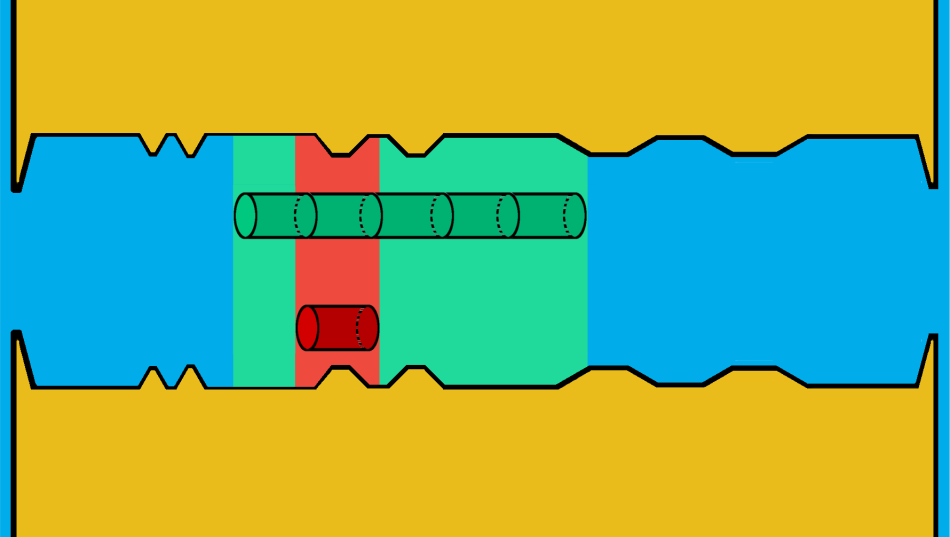
\includegraphics[height=1.05in]{rod_convolution.png}
		\hspace{.1in}
		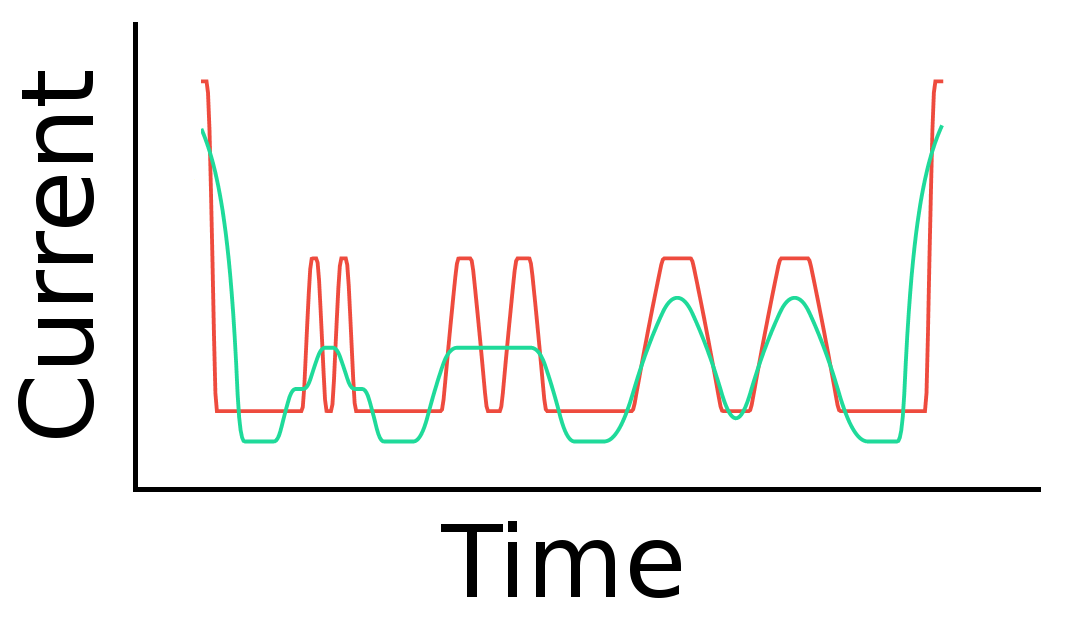
\includegraphics[height=1.25in]{rod_simulated_labeled.png}
		\par
	}
	
\end{frame}



%%%%%%%%%%%%%%%%%%%%%%%%%%%%%%%%%%%%%%%%%%%%%%%%%%%%%%%%%%%%%%%%%%%%%%%%%%%%%%%%%%%%%%%%%%%%%%%%%%%%%%%%%%%%%%%%%%%%%%%%%%%%
% Length measurement experimental platform
%%%%%%%%%%%%%%%%%%%%%%%%%%%%%%%%%%%%%%%%%%%%%%%%%%%%%%%%%%%%%%%%%%%%%%%%%%%%%%%%%%%%%%%%%%%%%%%%%%%%%%%%%%%%%%%%%%%%%%%%%%%%

\begin{frame}[c]{Length measurement experimental platform}
	\begin{itemize}
		\item Resistive pulses can be seen as a map of the pore interior for pores with non-constant radius
		\item In regions of low diameter, the pulse is deeper; in large diameter regions, the pulse is shallow
		\item Particles shorter than the length scale of diameter variation accurately map the pore interiors
		\item Particles longer than the length scale of diameter variation create RP signals that can be seen as a convolution of the pore's interior shape
	\end{itemize}
	
	\begin{equation}
		\begin{split}
			 \Delta R = R_{p}-R_{0} &= \rho\int_{z=0}^{z=l_{P}}\frac{dz}{A\left(z\right)}-\rho\int_{z=0}^{z=l_{P}}\frac{dz}{A'\left(z\right)} \\ 
			 &= \rho\int_{z=z'-l_{p}/2}^{z=z'+l_{p}/2}\frac{1}{\pi\left[r_{P}^{2}\left(z\right)-r_{p}^{2}\left(z\right)\right]}-\frac{1}{\pi r_{P}^{2}\left(z\right)}
		\end{split}
	\end{equation}

\end{frame}

\end{document}

